\chapter{Diseño}
\label{cap:capitulo4}

En este capítulo se expone, de forma detallada, el proceso seguido para conseguir que un dron detecte y navegue autónomamente hacia una señal \ac{RF}. Además, se muestra el desarrollo de una aplicación responsiva, que simula el comportamiento de una señal (en un espacio libre de obstáculos), basada en la aproximación de Friis. A continuación, en la figura~\ref{fig:diagrama}, se muestra un diagrama de bloques donde se ve una panorámica del sistema empleado.\\

\begin{figure} [t]
	\begin{center}
	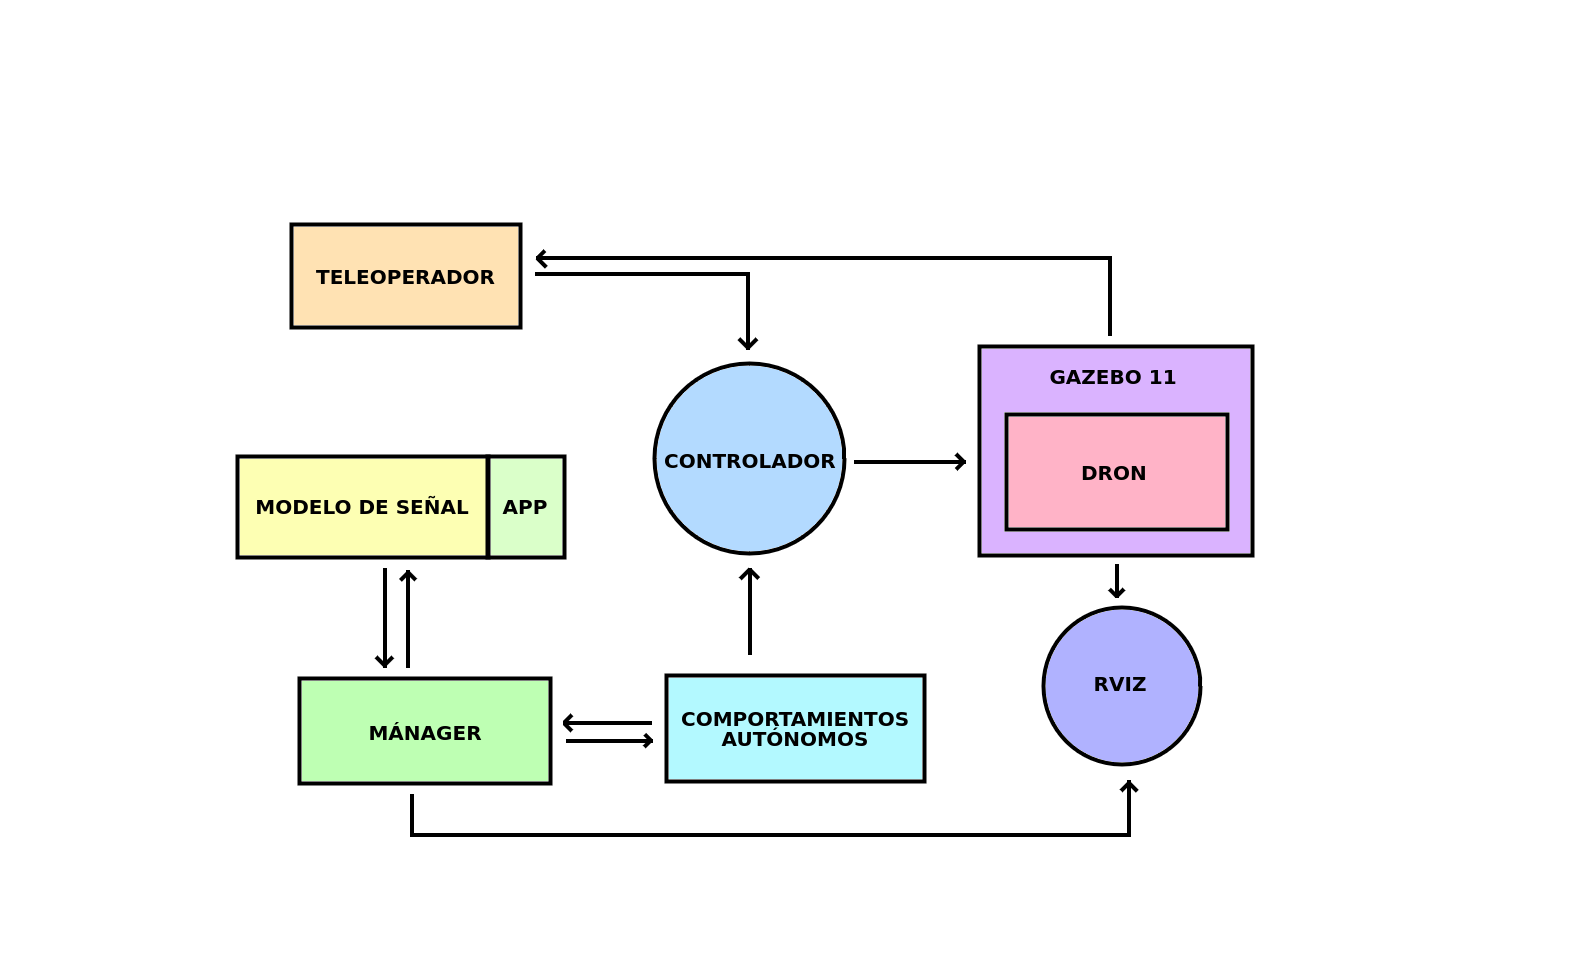
\includegraphics[height=10cm]{imagenes/cap4/0_diagrama_general.png}
	\end{center}
	\caption[Diagrama esquemático del sistema completo]{Diagrama esquemático del sistema completo}
	\label{fig:diagrama}
\end{figure}

Tal y como se puede apreciar, se tiene un controlador, encargado de comandar órdenes al dron; un simulador, que nos permite visualizar el modelo y el comportamiento del dron; el propio dron, que devuelve datos a otros bloques, tales como su posición o la imagen de la cámara instalada, entre otros; Rviz, como bloque de depuración y visualización; \ac{MPSS}, encargado de gestionar la transmisión de información del bloque de algoritmos de navegación autónoma y Rviz, a través del modelo de propagación de señal; bloque de comportamientos autónomos, que almacena la algoritmia responsable de resolver la navegación autónoma hacia el transmisor de la señal \ac{RF}; y por último, el bloque de teleoperación, el cual se encarga de solicitar órdenes al controlador para desencadenar acciones en el dron, tales como desplazamientos y giros.

\section{Preparación del entorno}
\label{sec:preparacion_del_entorno}

Inicialmente, se pone en funcionamiento el entorno de simulación (compatible con \ac{ROS}), así como el sistema de control de versiones, para mantener la trazabilidad y los backups. Por ello, se crea un repositorio común en GitHub y se instala y prueba el paquete de herramientas dispuesto por JdeRobot.

\subsection{JdeRobot - drones}
\label{subsec:jderobot_drones}

Gracias a esta plataforma, se obtienen los modelos y módulos necesarios para simular en Gazebo 11 un cuadracóptero, provisto de un sistema autopilot PX4. Específicamente, el modelo usado es el 3DR Iris simulado, con un plugin de una cámara frontal, el cual se ha incluido manualmente en el fichero original, debido a que el modelo específico disponible no funcionaba correctamente. Este dispositivo utiliza MAVROS para realizar la comunicación, lo que nos permite enviar y recibir mesajes ROS compatibles con el protocolo de comunicaciones típico de estas aeronaves, MAVLink.\\

\begin{figure} [t]
	\begin{center}
	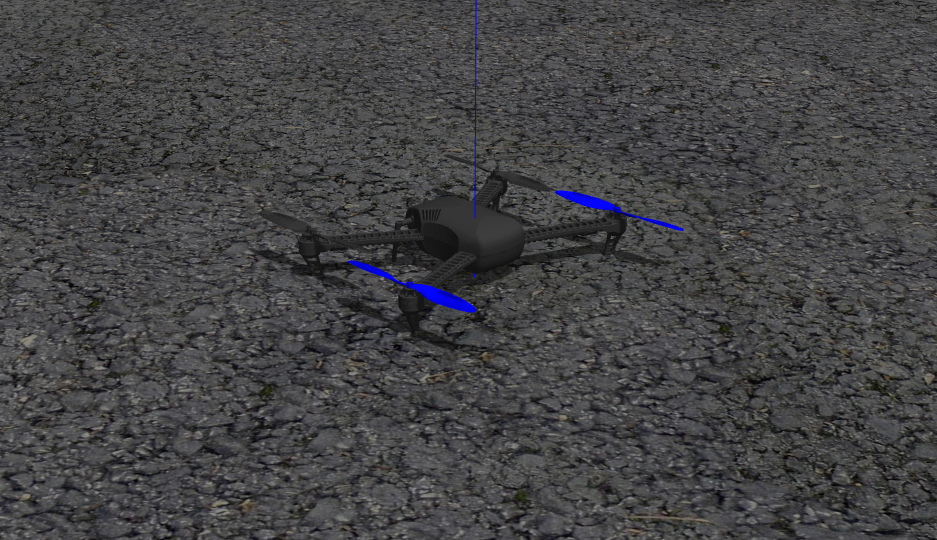
\includegraphics[height=6cm]{imagenes/cap4/1_px4_drone_gz.png}
	\end{center}
	\caption[3DR Iris simulado]{3DR Iris simulado}
	\label{fig:3dr_iris}
\end{figure}

\subsection{Teleoperador}
\label{subsec:teleoperador}

Una vez es funcional el entorno y los modelos, la primera aproximación ha consistido en realizar una interfaz gráfica, para enviar órdenes a la aeronave a modo de teleoperador. Para ello, se debe conseguir enviar mensajes de forma programática. Por tanto, se diseña un script controlador encargado de la comunicación directa con el controlador de la aeronave, que a su vez se encarga enviar y recibir diversos datos vía MAVROS. De igual modo, se satisfacen una serie de requisitos para asegurar el correcto funcionamiento del sistema:

\begin{enumerate}
	\item La comunicación se debe dar a más de 2 Hz, para evitar cambios indeseados en el funcionamiento interno del controlador PX4 (de la aeronave).
	\item Antes de realizar cualquier comunicación, se debe asegurar que el estado es \emph{``connected''}, lo que significa que el dron esta armado y en modo \emph{OFFBOARD} (nuestra aeronave posee 7 modos distintos, \emph{HOLD}, que mantiene la posición, \emph{RETURN}, que vuelve al punto de despegue, \emph{MISSION}, que permite cargar rutas programadas con anterioridad, \emph{TAKEOFF}, habilita el despegue, \emph{LAND}, habilita el aterrizaje, \emph{FOLLOW ME}, que permite seguir objetivos, y \emph{OFFBOARD}, que permite comandar al dron sin necesidad de GPS, lo que es útil de cara al desarrollo de aplicaciones robóticas)\footnote[1]{\url{https://docs.px4.io/main/en/getting_started/flight_modes.html}}.
    \item Una vez está conectado, se deben enviar velocidades al controlador PX4, con el fin de evitar el cierre de la conexión. Estos datos carecen de utilidad más que la de asegurar dicha conectividad.
    \item Por último, y antes de enviar cualquier posición, velocidad o comando (distintos modos de actuación), se debe comprobar siempre que el modo activo es \emph{OFFBOARD} y que el dron esta armado (listo para volar). En caso contrario, se debe solicitar al controlador, mediante servicios, dichos requerimientos.
\end{enumerate}

Por tanto, la manera de generar comportamientos en el dron en sí, es mediante \emph{topics}. Concretamente, los que genera MAVROS automáticamente cuando se lanza todo el sistema. Tal y como se comentó en apartados anteriores, estos \emph{topics} sólo admiten mensajes \ac{ROS}, lo que encapsula el mensaje real transmitido al controlador PX4, que solo es compatible con MAVLINK. En nuestro caso, se envían posiciones (PoseStamped), velocidades (Twist) y comandos (sevicios formados por mensajes personalizados, creados por MAVROS, con formato \ac{ROS}, como por ejemplo aterrizar). Esto, nos permite conectar el resto de aplicaciones con el script controlador, mediante \emph{topics} comunes, es decir a través de \emph{``radio\_control/[pos, vel o cmd]''}, de forma de que el script controlador se encargue de enviar la acción final al dron, empleando los \emph{topics} propios de MAVROS, vease \emph{``mavros/setpoint\_position/local''} (que solicita al dron una posición en coordenadas del simulador), \emph{``mavros/setpoint\_velocity/cmd\_vel\_unstamped''} (que de igual modo solicita velocidades), \emph{``mavros/cmd/land''} (para solicitar el aterrizaje), \emph{``mavros/cmd/arming''} (para armar el dron, o dicho de otro modo, para que el dron este listo para actuar), y por último \emph{``mavros/setmode''} (para solicitar un modo de actuación determinado). Para más detalle, mirar la figura~\ref{fig:diagrama2}, donde se especifican los tipos de mensaje enviados de forma gráfica.\\

\begin{figure} [t]
	\begin{center}
	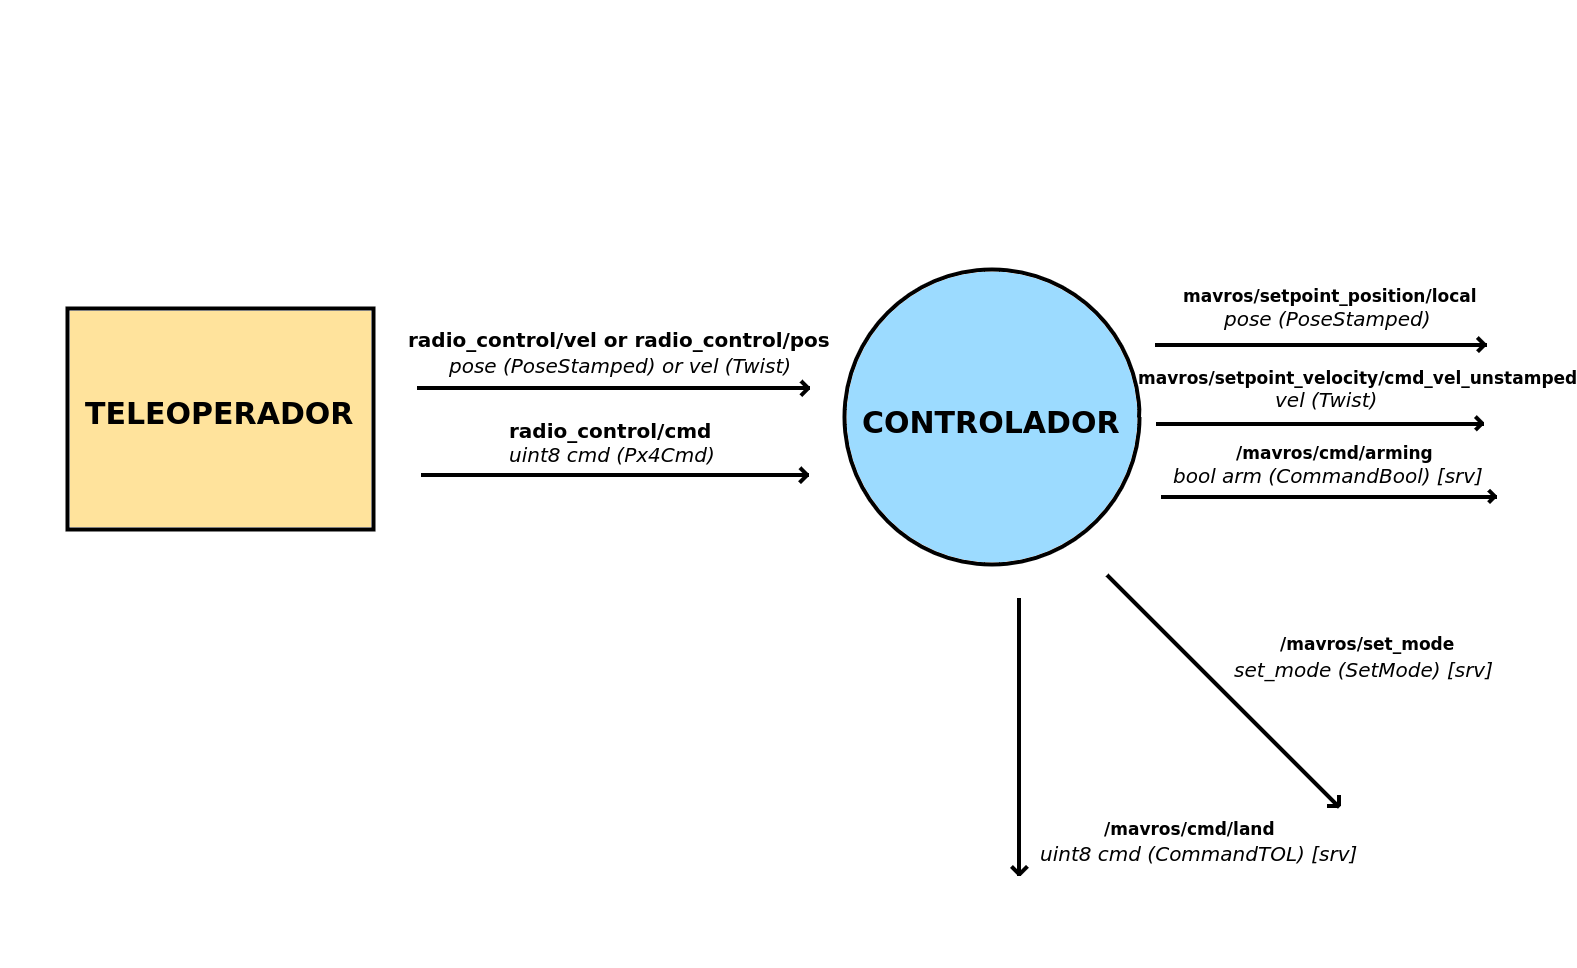
\includegraphics[height=10cm]{imagenes/cap4/4_esquema_coms.png}
	\end{center}
	\caption[Esquema comunicaciones del controlador]{Esquema comunicaciones del controlador}
	\label{fig:diagrama2}
\end{figure}

De este modo, el teleoperador se diseña con el fin de generar comportamientos que se usarán en las fases finales del \ac{TFG}. Sin embargo, para la primera versión, tan solo se construye una interfaz gráfica, encargada de enviar ordenes usando \ac{ROS} que, en última instancia, llegan al dron y producen diversos comportamientos, tales como moverse y girar, a través de barras de acción.\\

En la siguiente versión, se programan comportamientos predefinidos, es decir, acciones predeterminadas tales como desplazarse distancias concretas en ciertas direcciones, o girar un número específico de grados en un sentido u otro. Para ello, se diseña una ampliación sobre la interfaz anterior, en la que se añade un botón por cada acción concreta desarrollada, además de una imagen de la cámara frontal en tiempo real.\\

Por último, se simplifica la interfaz, con el fin de seleccionar los comportamientos más relevantes de cara al proyecto. Además, se agregan marcadores en \emph{rviz}, para determinar las celdas visitadas (con colores aleatorios), junto con otro marcador que muestra la trayectoria que sigue la aeronave, como se puede observar en la figura~\ref{fig:teleop_figs}.\\

\begin{figure} [t]
	\centering
	\subfigure[Primera versión]{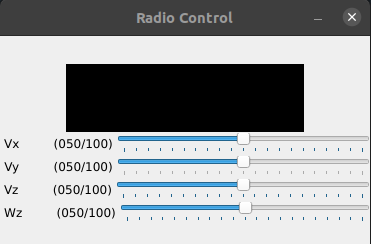
\includegraphics[height=5.5cm]{imagenes/cap4/2_axes_rc.png}}
	\quad
	\subfigure[Versión final]{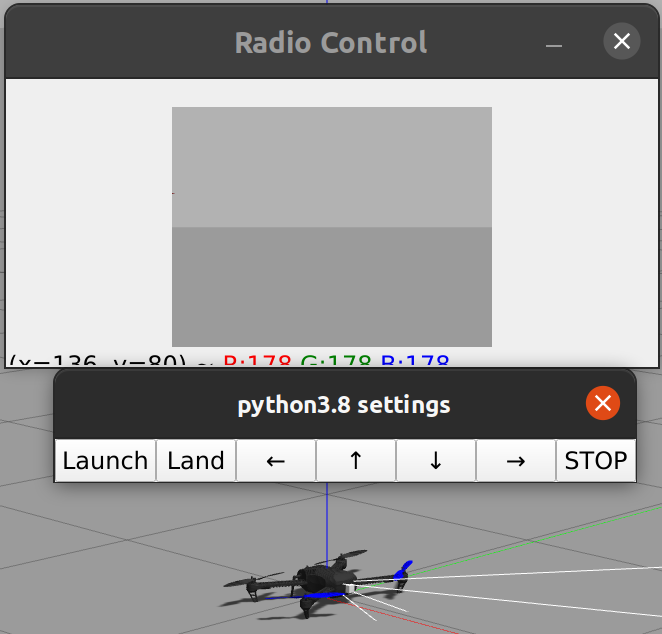
\includegraphics[height=5.5cm]{imagenes/cap4/3_c2c_gui.png}}
    \quad
    \subfigure[Marcadores Rviz]{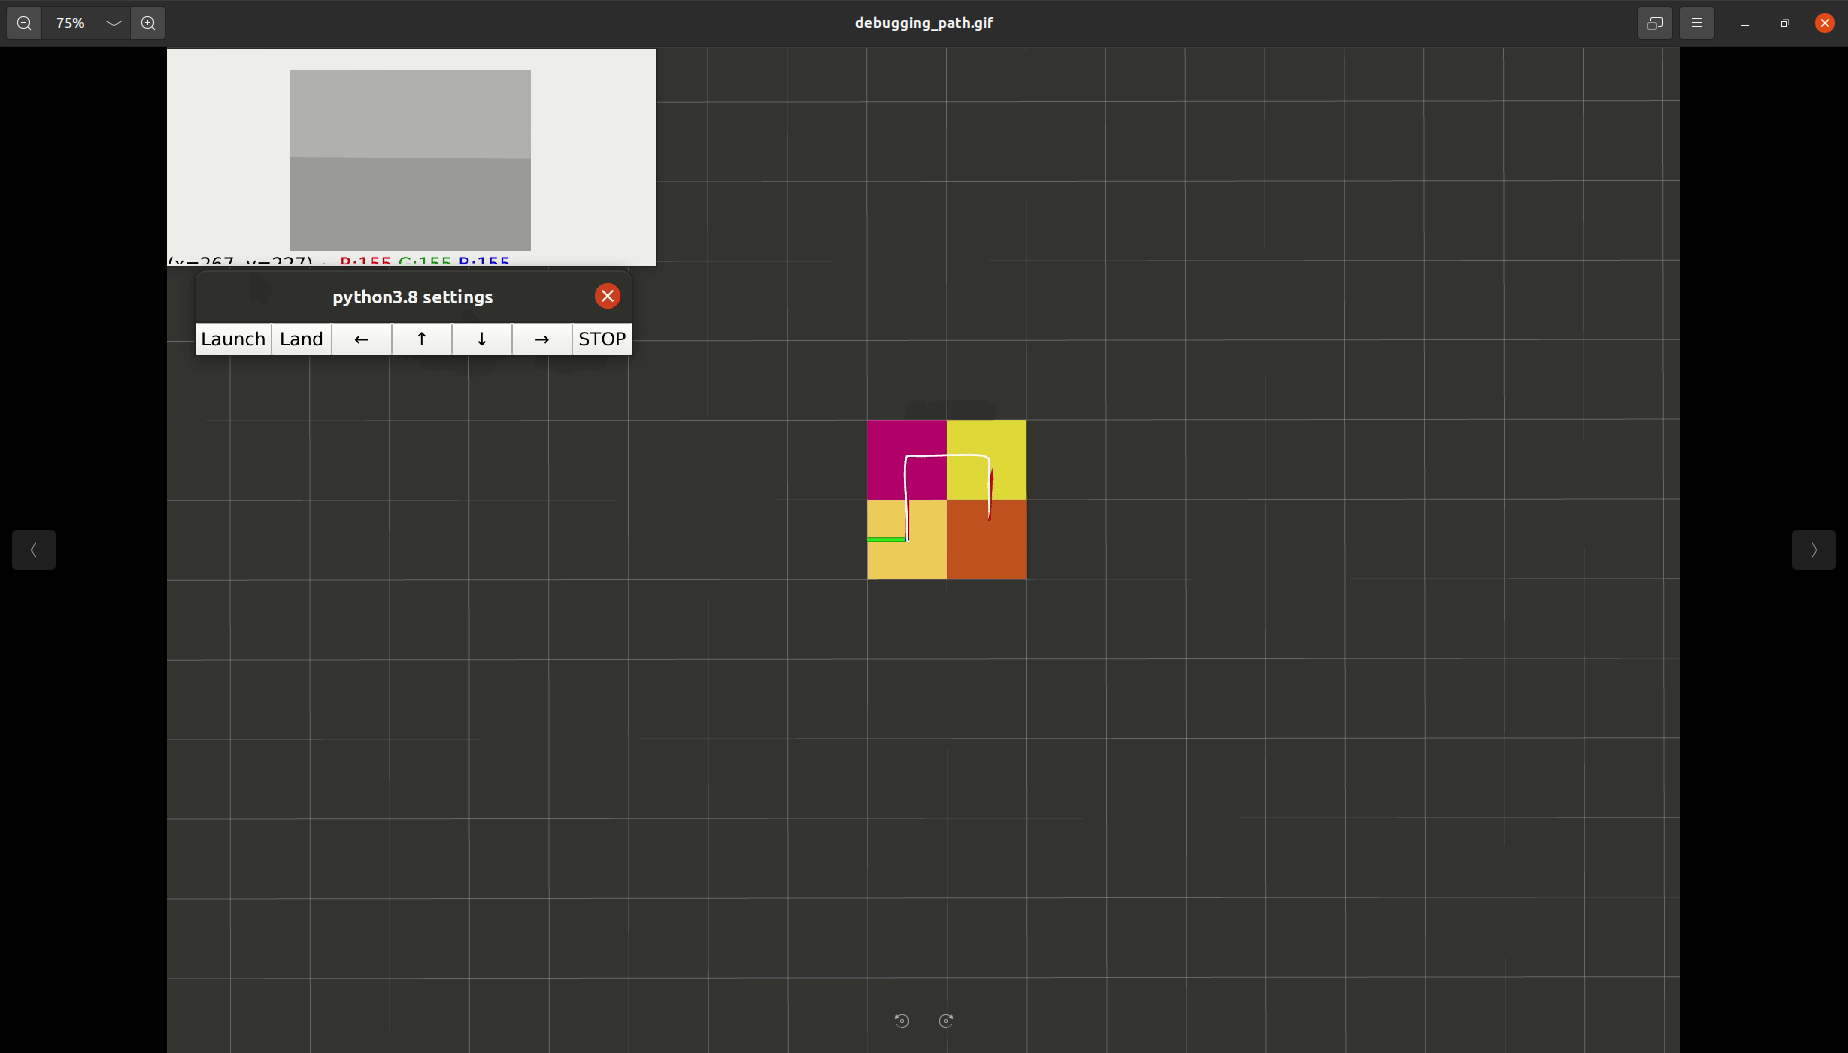
\includegraphics[height=8.5cm]{imagenes/cap4/3_rviz_path.png}}
	\caption{Teleoperador}
	\label{fig:teleop_figs}
\end{figure}

A continuación, en el código~\ref{cod:c2c_app}, se muestra la última versión comentada de la interfaz. En este caso se muestra el \emph{``main''}, donde, tras inicializar el nodo \ac{ROS}, se definen por un lado los suscriptores, encargados de recibir los datos de la cámara y la posición del dron (usando MAVROS), los publicadores, cuya función es enviar posiciones y/o comandos al script controlador, y por último la interfaz gráfica diseñada con OpenCV, donde se define la ventana y los botones con las diversas acciones predefinidas\footnote[2]{Código completo en \url{https://github.com/RoboticsLabURJC/2022-tfg-cristian-sanchez/blob/main/src/teleop/scripts/c2c_control.py}}.\\

\begin{code}[t]
\begin{lstlisting}[language=Python]
if __name__ == '__main__':
    try:
        rospy.init_node(NODENAME, anonymous=True)

        # Msgs
        ## Subscribers
        image_sub = rospy.Subscriber(IMAGE_TOPIC, Image, callback = image_cb)
        current_pos_sub = rospy.Subscriber(LOCAL_POSE_TOPIC, PoseStamped, callback = current_pos_cb)

        ## Publishers
        pos_pub = rospy.Publisher(RADIO_CONTROL_POS_TOPIC, PoseStamped, queue_size=10)
        cmd_pub = rospy.Publisher(RADIO_CONTROL_CMD_TOPIC, Px4Cmd, queue_size=10)

        # -- OPENCV -- #
        cv2.namedWindow(WINDOWNAME)

        # Buttons
        cv2.createButton('Launch', launch_button, None, cv2.QT_PUSH_BUTTON, 1)
        cv2.createButton('Land', land_button, None, cv2.QT_PUSH_BUTTON, 1)
        cv2.createButton('←', left_button, None, cv2.QT_PUSH_BUTTON, 1)
        cv2.createButton('↑', front_button, None, cv2.QT_PUSH_BUTTON, 1)
        cv2.createButton('↓', back_button, None, cv2.QT_PUSH_BUTTON, 1)
        cv2.createButton('→', right_button, None, cv2.QT_PUSH_BUTTON, 1)
        cv2.createButton('STOP', stop_button, None, cv2.QT_PUSH_BUTTON, 1)

        cv2.waitKey(0)
        cv2.destroyAllWindows()
    except rospy.ROSInterruptException:
        pass
\end{lstlisting}
\caption[Bloque de código principal de la versión final del teleoperador]{Bloque de código principal de la versión final del teleoperador}
\label{cod:c2c_app}
\end{code}

\section{Modelo de propagación de señal}
\label{sec:signals}

El siguiente paso consiste en generar un modelo de propagación de señales \ac{RF}. Este apartado es especialmente relevante, ya que nos permite desarrollar una aplicación reactiva, con la idea de generar entornos en tiempo real que simulan la propagación de una señal, sobre la que probar nuestras soluciones. Para entender bien todo, dejo una referencia en el anexo~\ref{cap:anexo} con una serie de conceptos introductorios últiles para abordar esta sección.\\

En cuanto al modelo de propagación de señal, se define como un modelo que nos ayuda a calcular de que manera se propaga una señal por el aire, en función de la potencia, frecuencia, distancia y entorno, entraremos en detalle a continuación. La idea es implementar el modelo e integrarlo en \ac{ROS}, ya que no hay nada desarrollado y de cara a resolver problemas de este tipo, puede ser realmente útil.\\

\subsection{Aproximación de Friis}
\label{subsec:friis}

Para ello, se opta por emplear la aproximación de Friis, presentada por el ingeniero Danés-Americano Harald T. Friis en 1946, el cual buscaba una manera de medir el rendimiento de una antena \cite{johnson1984antenna}. De este modo, nos ofrece la siguiente ecuación para modelar nuestro problema:

\begin{align}
    P_r = P_t \cdot \left( \frac{G_t G_r \lambda^2 }{(4 \pi)^2 d^n L} \right)
\end{align}

Donde cada término significa lo siguiente\footnote[3]{\url{https://www.gaussianwaves.com/2013/09/friss-free-space-propagation-model/}}:

\begin{enumerate}
    \item \emph{$P_t$ y $P_r$}: aluden a la potencia del transmisor y la potencia del receptor respectivamente.
    \item \emph{Ganancias} ($G_t$, $G_r$): representan un valor incremental aplicado a la potencia de emisión y de recepción, respectivamente.
    \item \emph{Valor lambda} ($\lambda$): hace referencia a la longitud de onda. Está directamente relacionado con la frecuencia.
    \item \emph{Distancia} (d): desde el origen de la señal a un punto en el espacio.
    \item \emph{L}: representa todas aquellas pérdidas no asociadas a la propagación de la señal.
    \item \ac{PLE} (n): permite ajustar el modelo a diversos entornos. Es un valor constante extraido de forma empírica. Como se puede observar en la figura~\ref{table:ple_table}.
\end{enumerate}

\begin{table} [t]
    \centering
    \begin{tabular}{ll}
    \textbf{Entorno}            & \textbf{Exponente n} \\
    Sin obstáculos              & 2 \\
    Zona urbana                 & 2'7 a 3'5\\
    Zona urbana densa           & 3 a 5  \\
    Interior (a la vista)       & 1'6 a 1'8 \\
    Interior (obstaculizado)    & 4 a 6 \\
    Almacen (obstaculizado)     & 2 a 3 \\
    \end{tabular}
    \caption[Valores n de referencia]{Valores n de referencia}
    \label{table:ple_table}
\end{table}

Además, empleando este método, podemos modelar las pérdidas de una señal estimadas durante su propagación, a través de la siguiente ecuación:\\

\begin{align}
    P_L(dB) = -10 \log_{10} \frac{\lambda^2}{(4 \pi d)^2}
\end{align}

\subsection{Módulo python de Friis}
\label{subsec:friis-module}

Una vez desarrollado lo anterior, lo siguiente consiste en encontrar la forma de que todo esto sea accesible para cualquier aplicación que lo desee en el ecosistema Python. Debido a esto, surge la idea de crear un módulo python encargado de modelar las ecuaciones previamente mencionadas. Para ello, se diseña una clase cuyo constructor recibe, por parámetros, las variables implicadas en las ecuaciones de Friis, además de las dimensiones del mapa y su resolución (la cual afecta al tamaño de celda).\\

Básicamente, el proceso a seguir para usar este módulo es el siguiente, primero se crea un objeto de la clase Friis donde se especifican las características de la señal y las variables relacionadas, lo que genera internamente un array 2D vacío, que será rellenado en función de la configuración seleccionada. Posteriormente, se selecciona el modelo deseado (propagación o pérdidas), pasando las coordenadas del origen de la señal por parámetros. Esto, retornará el array relleno con los valores de potencia asociados a las ecuaciones del modelo de Friis seleccionado. A continuación, en el código~\ref{cod:friis_basics}, se muestra un ejemplo de uso sencillo, donde se obtiene un mapa de propagación de señal, en forma de Numpy array 2D:

\begin{code}[H]
    \begin{lstlisting}[language=Python]

    #! /usr/bin/env python
    import friss as fr

    if __name__ == '__main__':
        friis_object = fr.Friss(power_tras=10.0,
                                gain_tras=1.5,
                                gain_recv=2.0,
                                freq=fr.FREQ_WIFI,
                                losses_factor=1.0,
                                losses_path=2.0,
                                world_sz=(10,10),
                                resolution=1.0)

        signal_map = friis_object.model_power_signal(origin=(5,3))

\end{lstlisting}
\caption[Ejemplo básico de uso del módulo Friis]{Ejemplo básico de uso del módulo Friis}
\label{cod:friis_basics}
\end{code}

Concretamente, se genera un array 10x10 con resolución 1 (es decir, representa celdillas de 1x1 metros), de una señal WIFI (2'4 GHz), donde el transmisor emite a 10 W, con una ganancia de 1.5, el receptor posee una ganancia de 2, un factor de pérdidas (L) de 1, es decir, sin pérdidas, y por último, el exponente n (\ac{PLE}) con un valor de 2, que representa el espacio vacío. Luego se genera el modelo de propagación de la señal, indicando que la fuente se encuentra en las coordenadas (5,3). En la figura~\ref{fig:heat_ex}, se muestra una representación del código~\ref{cod:friis_basics}, pero para un mapa de mayor dimensión (50 x 50 metros), de modo que se aprecie mejor las diferencias entre unos y otros.\\

\begin{figure} [t]
	\begin{center}
	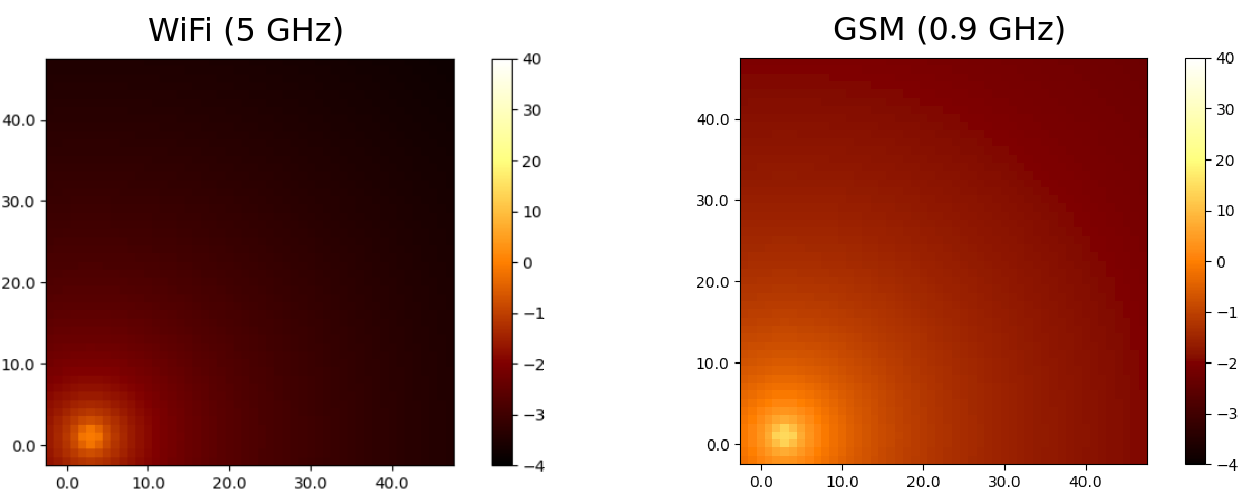
\includegraphics[height=6cm]{imagenes/cap4/4_heatmap_example.png}
	\end{center}
	\caption[Uso del módulo Friis con señal WIFI (2'4 Ghz) VS señal GSM (0'9 GHz)]{Uso del módulo Friis con señal WIFI (2'4 Ghz) VS señal GSM (0'9 GHz)}
	\label{fig:heat_ex}
\end{figure}

Adicionalmente, este módulo posee otras funcionalidades útiles para trabajar con él, como son:

\begin{enumerate}
    \item \emph{reset\_world}: modifica el mapa que hubiera, estableciendo todos sus valores a cero.
    \item \emph{get\_world\_sz}: retorna las dimensiones del mapa.
    \item \emph{set\_values}: modifica las características de la señal simulada.
\end{enumerate}

Hay que tener en cuenta que, aunque se modifiquen los parámetros, se debe modelar de nuevo el mapa para que surtan efectos los cambios.\\

\subsection{Aplicación de Friis}
\label{subsec:friis-app}

Finalmente y agrupando lo anterior, se integra el módulo previo, en una interfaz gráfica intuitiva que ha servido para depurar. La idea es estudiar, en tiempo real, como evoluciona la señal cuando algunos de sus parametros, en la ecuación de Friis, son modificados.\\

Para ello, se emplea la librería matplotlib, debido a la enorme funcionalidad que dispone, así como de su sencillez a la hora de crear nuevas aplicaciones. Funciona de manera que se generan eventos que son gestionados en \emph{``callbacks''}, es decir, se generan bucles asociados a dichos eventos, que reaccionan a cambios en la interfaz generada. En nuestro caso, la estructura base consta de una figura, sobre la que se agregan todos los elementos, entre los que encontramos los mapas de calor o \emph{``heatmap''} en forma de plots, las barras de acción o \emph{``sliders''}, botones, entre otros elementos que se explicarán más adelante.\\

Inicialmente, se opta por representar un mapa de calor con una barra de color asociada a los distintos valores de la señal. Además, se integran sliders correspondientes a cada valor presente en la ecuación de Friis. El problema es, que al actualizar los valores, también lo hace la representación, por lo que no se aprecia el efecto de los cambios en el plot. Por ello, se decide agregar dos mapas de calor, uno con el máximo y el mínimo fijados a mano (donde sí se aprecian los cambios), y el anterior mencionado. Para elegir cual usar, se añade una casilla marcable. Además, se incluyen dos variables relevantes a la hora de modelar, el tamaño del mapa y la resolución, manejadas a través de \emph{``sliders''}, los cuales a su vez se activan al pulsar un botón de SET, que recarga la interfaz. Además, se ajustan los saltos de valores para que sean coherentes en el resto de barras de acción, tal y como se puede apreciar a continuación:\\

\begin{figure} [t]
    \begin{center}
    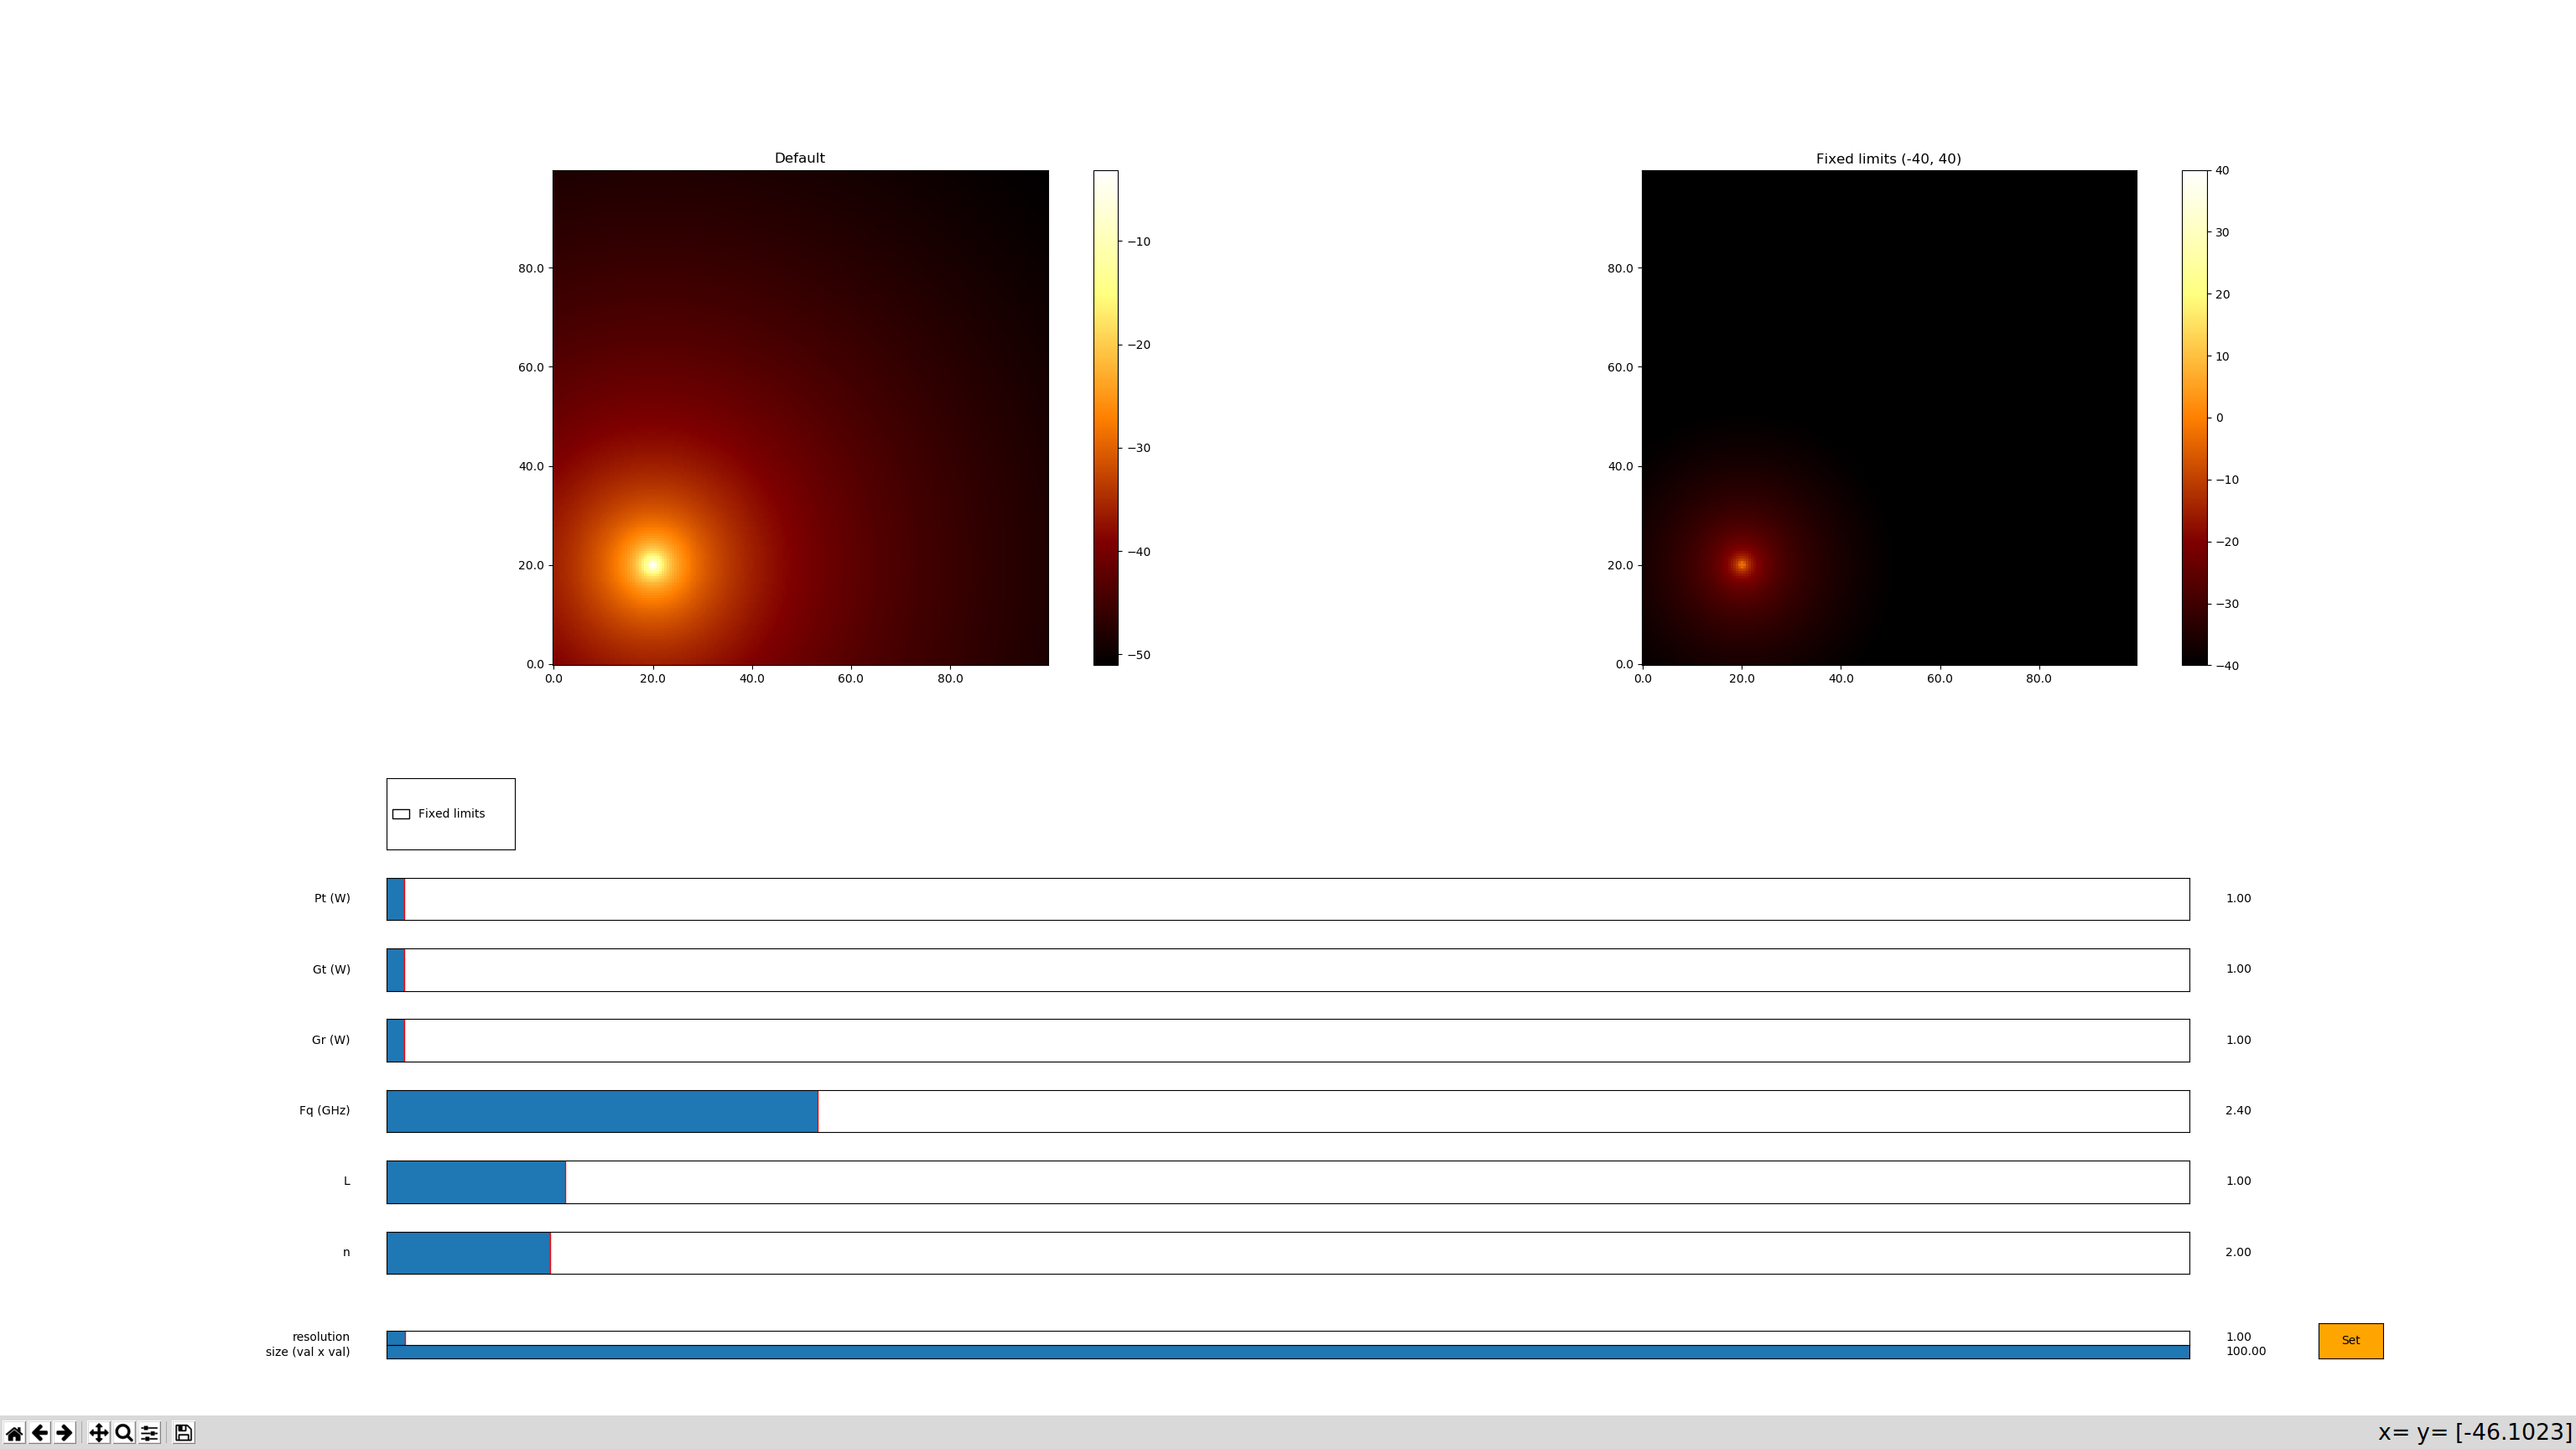
\includegraphics[height=8cm]{imagenes/cap4/7_Friss_endGUI.png}
    \end{center}
	\caption[Versión final de la interfaz]{Versión final de la interfaz}
	\label{fig:friis_end_app}
\end{figure}

\subsection{\ac{MPSS} - Integración de Friis con \ac{ROS}}
\label{subsec:friis-ros}

\begin{figure} [t]
    \begin{center}
    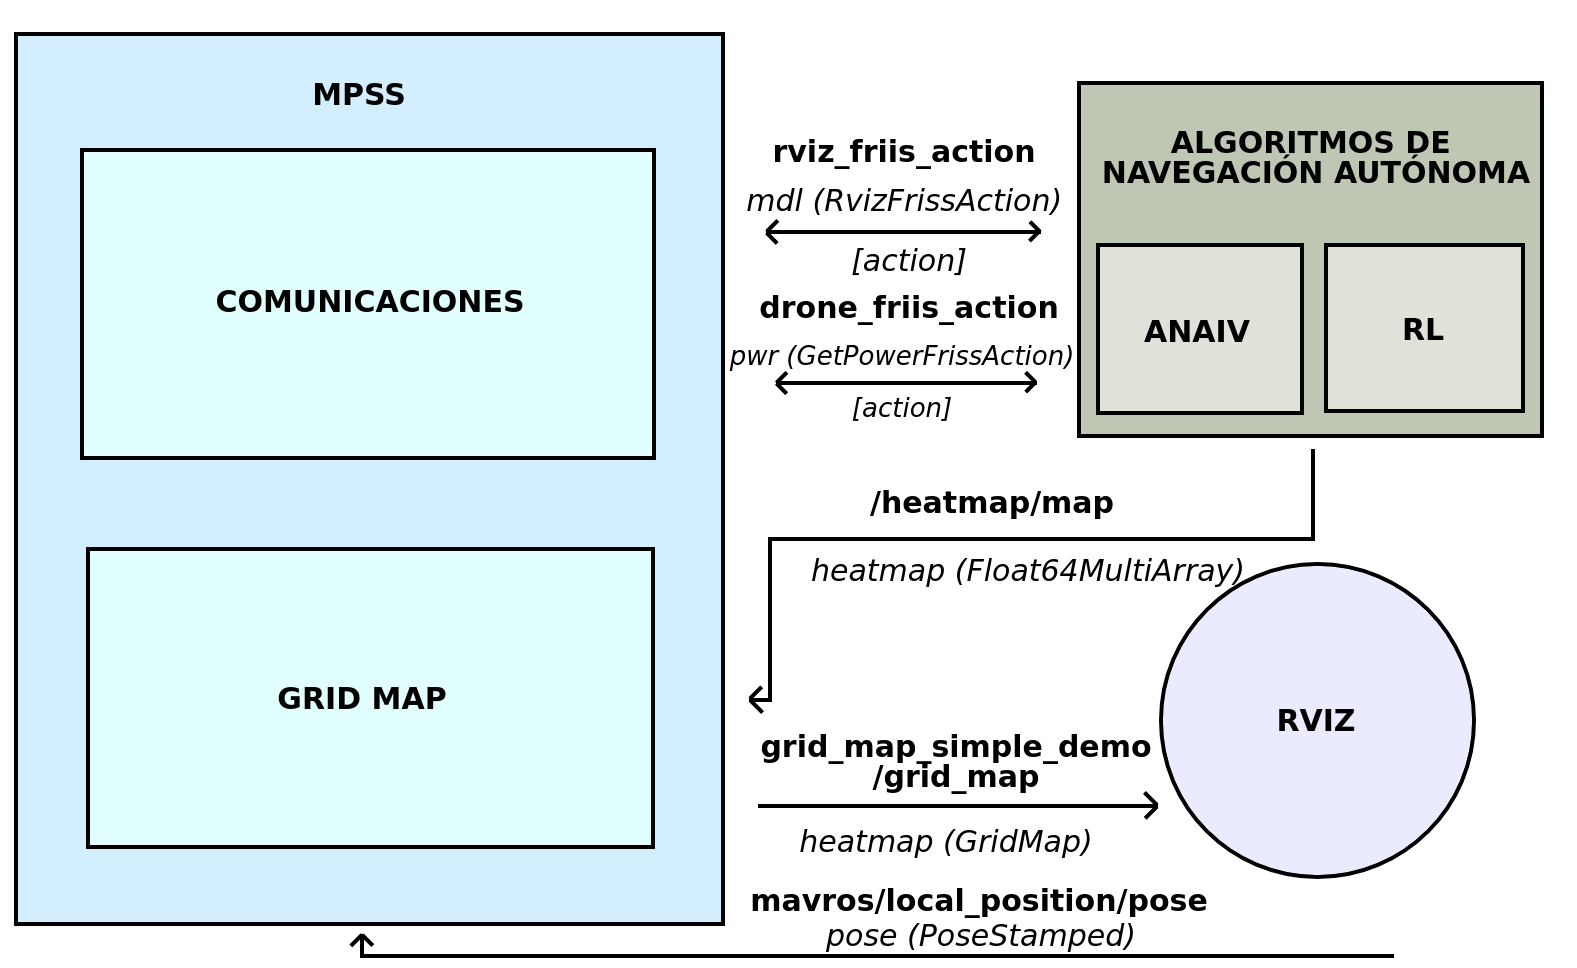
\includegraphics[height=8cm]{imagenes/cap4/5_MPSS_esquema.png}
    \end{center}
	\caption[Esquema comunicaciones \ac{MPSS}]{Esquema comunicaciones \ac{MPSS}}
	\label{fig:esquema_mpss}
\end{figure}

Por último y cómo se comentó al inicio de la sección~\ref{sec:signals} y siguiendo el esquema de la figura~\ref{fig:esquema_mpss}, se ha diseñado una aplicación servidor de datos, que funciona como intermediaria entre el módulo de Friis y otros nodos \ac{ROS} (en este caso, con un diseño enfocado a simular de manera realista el escenario con el dron). Básicamente, la aplicación hace uso del módulo de Friis para gestionar la información que envía a según que aplicación. Este programa se compone de dos servidores basados en acciones \ac{ROS}, los cuales son especialmente útiles dada su naturaleza asíncrona. Dichos servidores, se encargan de las peticiones y respuestas para el dron y para rviz, tal y como se detalla a continuación:

\begin{enumerate}
	\item \emph{Bloque de comunicaciones}: en términos generales, el dron envía su posición en coordenadas transformadas al sistema de referencia del \emph{``heatmap''}, y recibe el valor de la señal de dichas coordenadas, mediante acciones \ac{ROS} (\emph{``drone\_friis\_action''}). En un caso real, el dron tan solo accedería al valor de la señal a través de un sensor que se lo permitiera. Adicionalmente, se le ha agregado la funcionalidad de enviar, en dicha petición, si se deseaba un mapa con obstáculos o no en la misma petición (de manera que \ac{MPSS} generase un modelo con obstáculos). En paralelo, recibe una petición para agregar todas las características de la señal y sobre la que generar el \emph{``heatmap''}, vease el origen y sus componentes. Esto, genera como respuesta un array de floats que contienen la información del mapa de calor, en un formato adecuado para su representación. Todo ello, nuevamente a través de acciones \ac{ROS}, en \emph{``drone\_friis\_action''}. De igual modo, ha sido agregada la funcionalidad de los obstáculos para la experimentación futura.
	\item \emph{Bloque grid map}: se encarga de transformar el mapa de calor en formato array, a un objeto compatible con la biblioteca grid\_map, que a través del topic de \ac{ROS} \emph{``heatmap/map''}, permite enviar los datos a un nodo que los transforma y reenvía a un plugin de rviz (usando el topic \emph{``grid\_map\_simple\_demo/grid\_map''}), el cual genera la representación visual buscada\footnote[4]{Toda la funcionalidad englobada en el directorio heatmap\_util del proyecto}.
\end{enumerate}

\section{Navegación autónoma para localizar el origen de una señal \ac{RF}}
\label{sec:signal_follow}

\subsection{Introducción al problema}
\label{subsec:intro_sf}

\begin{figure} [t]
    \begin{center}
    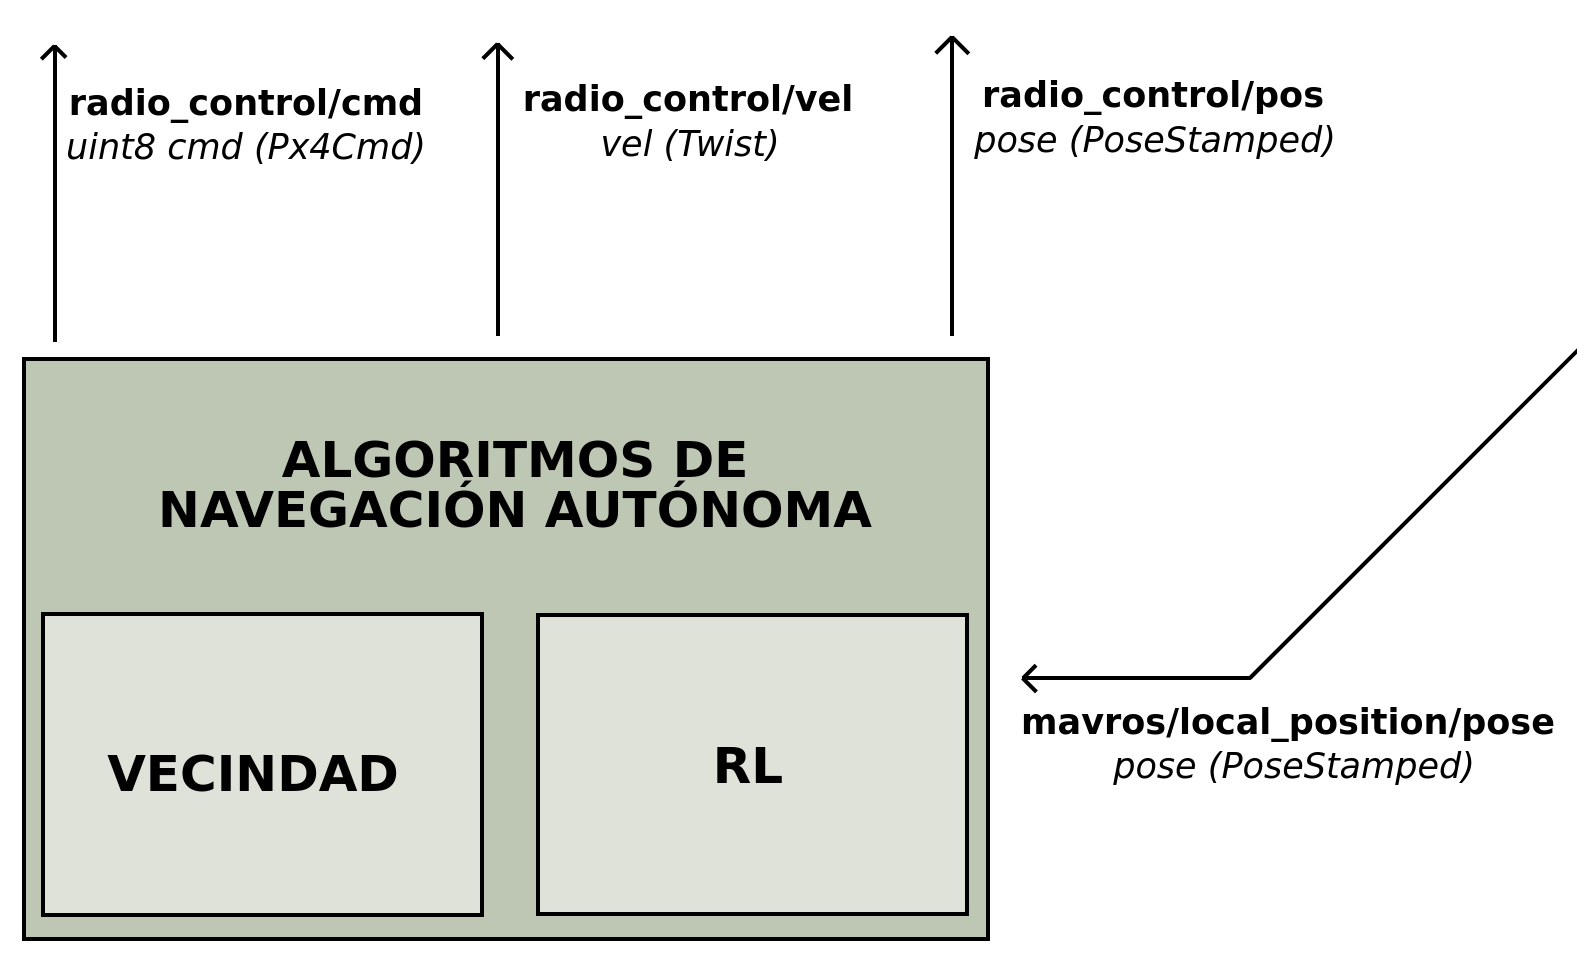
\includegraphics[height=8cm]{imagenes/cap4/5_esquema_comp_auto.png}
    \end{center}
	\caption[Esquema comunicaciones del bloque de comportamiento autónomo]{Esquema comunicaciones del bloque de comportamiento autónomo}
	\label{fig:esquema_auto}
\end{figure}

Tal y como se observa en la figura~\ref{fig:esquema_auto}, el bloque de algoritmos de navegación autónoma se comunica con el controlador para enviar las ordenes al dron, tal y como sucede con el teleoperador (vease sección~\ref{subsec:teleoperador}), enviando a través de los mismos \emph{topics} mencionados la información. Además se comunica con el \ac{MPSS}, tal y como se describió previamente en la figura~\ref{fig:esquema_mpss}. Adicionalmente y para el correcto funcionamiento de algunas funciones, recibe información de la posición del dron en el simulador a través del topic \emph{``mavros/local\_position/pose''}.

\subsection{\ac{ANAIV}}
\label{subsec:algoritmo_sf}

\begin{figure} [t]
    \begin{center}
    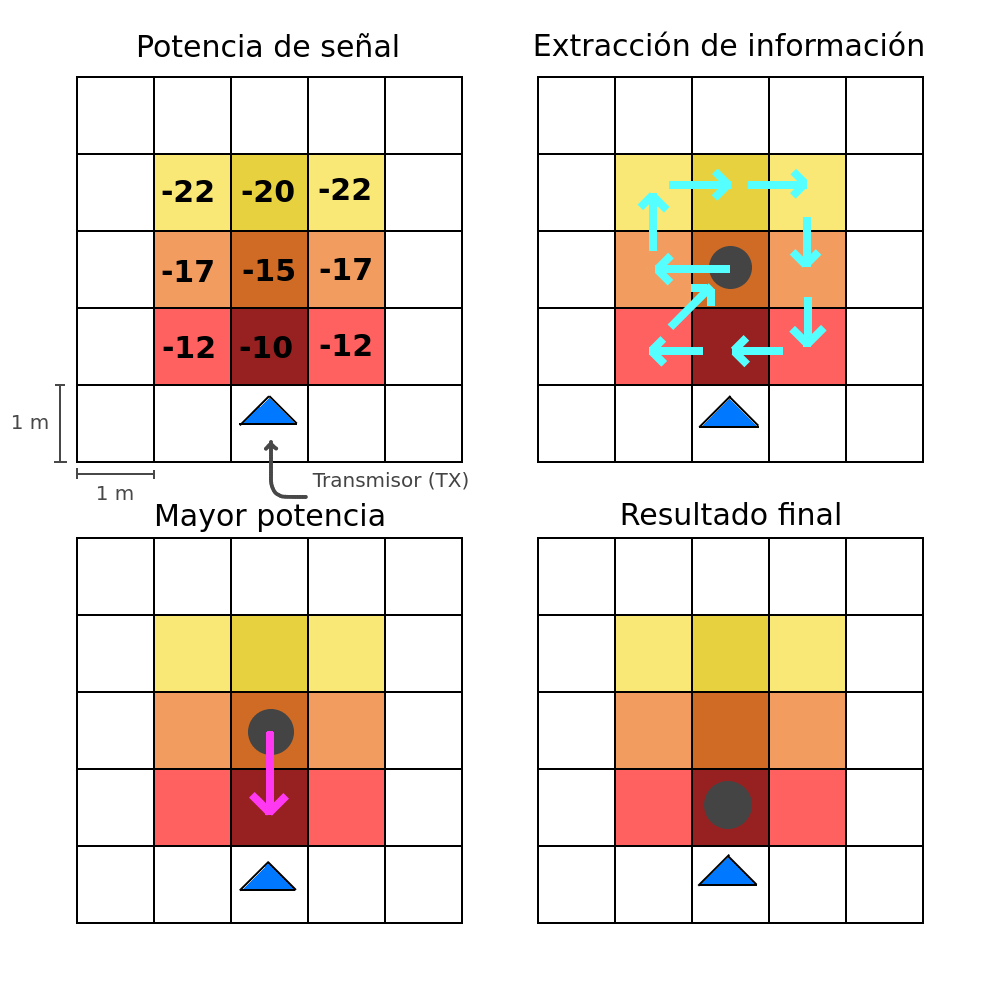
\includegraphics[height=12cm]{imagenes/cap4/9_algoritmo_manual.png}
    \end{center}
    \caption[Algoritmo de navegación autónoma basado en la información de la vecindad]{Algoritmo de navegación autónoma basado en la información de la vecindad}
    \label{fig:manual_algorithm}
\end{figure}

Antes de nada, dentro del bloque de algoritmos de navegación autónoma y como nexo de unión para cada algoritmo implementado, se parte de una clase \emph{``Drone''}, cuyo constructor se encarga de conectar los topics al controlador PX4 para comandar ordenes a la aeronave. Además, se encarga de establecer la comunicación con el servidor de datos (tanto para la potencia como para rviz) y define los diferentes atributos pertenecientes a la clase, que en este caso aluden a los parámetros necesarios para el funcionamiento de los algoritmos y la extracción de datos en los resultados, siguiendo esta estructura:

\begin{enumerate}
	\item \emph{Métodos para comandar al dron}: que se definen como el conjunto de funciones encargadas del movimiento del dispositivo (como despegar, aterrizar, desplazarse, entre otros). Mucha de esta funcionalidad ha sido adaptada del teleoperador comentado al de este capitulo.
    \item \emph{Métodos de tolerancia}: encargados de establecer un margen aceptable entre la posición del dron y el objetivo deseado. Estos métodos permiten controlar con precisión problemas que surgen de la deriva y de condiciones externas, como puede ser el viento.
	\item \emph{Métodos de conversión}: que permiten transformar las coordenadas entre los distintos sistemas de referencia presentes en el problema, tal y como se puede apreciar a continuación.
    \item \emph{Algoritmos}: o las soluciones \emph{``sigue señal''} propiamente dichas, que en sí, contienen el conjunto de métodos que cada cual necesita para llevarse a cabo. Se puede distinguir entre manual, manual optimizado y Q-Learning.
\end{enumerate}

Adicionalmente, se deben cumplir una serie de premisas de cara a la simulación. Estas son que, todos los movimientos realizados por el dron deben estar contenidos en el mapa de calor generado; además, la medida de la señal sólo podrá tomarse cuando el dron esté en el centro de la celda; los movimientos del dron deberán ser de centro en centro aunque esto abarque más celdas de distancia (problema resuelto y adaptado del teleoperador); y que la métrica de cada celda es de 1x1 metros.\\

Por ello, la primera aproximación se basa en visitar todos los vecinos más cercanos (un total de 9 posiciones) y realizar el movimiento que lleve a una posición con más potencia, tal y como se puede apreciar en la figura~\ref{fig:manual_algorithm}. Para ello, se toma la medida del sensor a bordo (simulado) en cada una de las posiciones vecinas disponibles, de donde se obtiene un valor en dB, de modo que las coordenadas candidatas para ser objetivo, son aquellas que posean mayor valor de señal. Posteriormente se realiza el desplazamiento y se repite el proceso hasta llegar a una condición de finalización o parada. En este caso, la condición de parada analiza si las coordenadas objetivo de la iteración anterior, son las mismas que las coordenadas objetivo de la iteración actual, cumpliendo además que todos los vecinos colindantes tienen un valor de la señal inferior al candidato a origen de la señal.\\

En cuanto a los métodos que se usan, se encuentra el de verificar movimientos válidos y el de comprobar si ha llegado a la casilla final, mediante la verificación anterior (vecindad con menor señal).\\

\subsection{\ac{ANAIV} (mejorado)}
\label{subsec:alg-manual-opt}

\begin{figure} [t]
    \begin{center}
    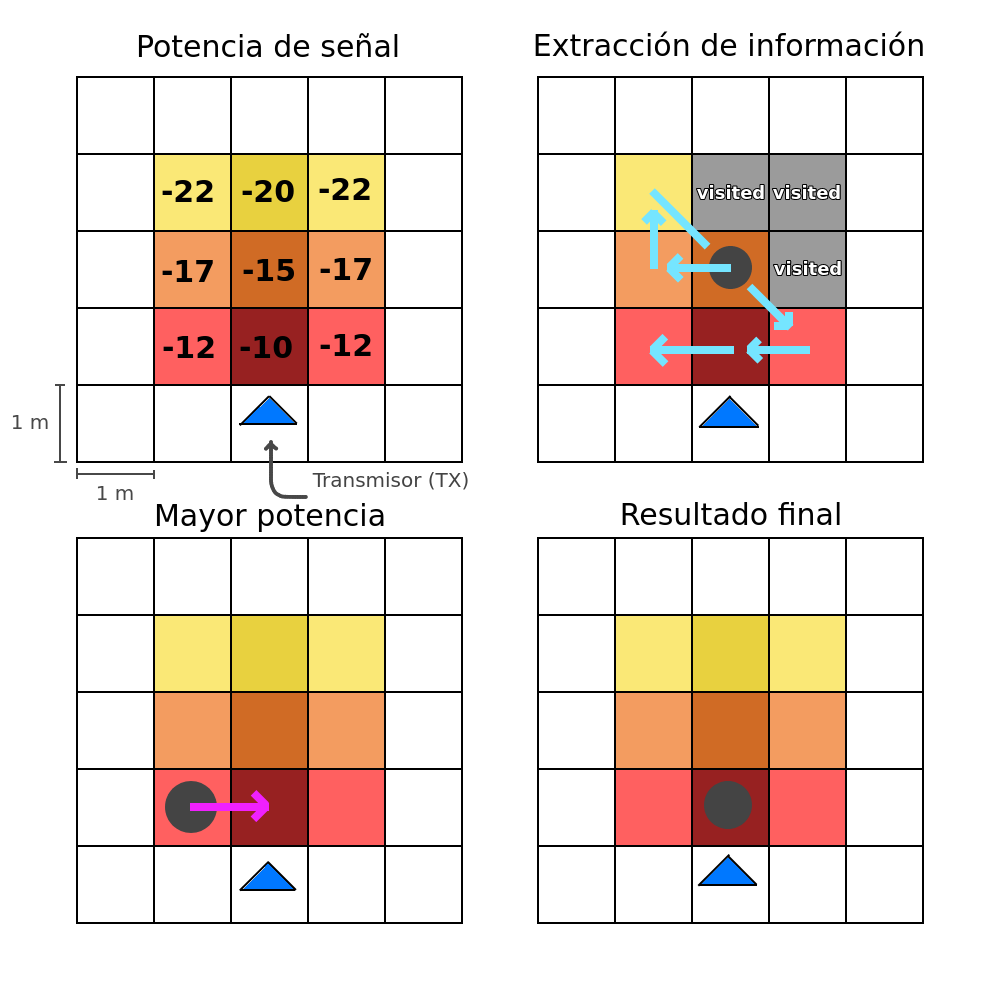
\includegraphics[height=12cm]{imagenes/cap4/10_algoritmo_optimizado.png}
    \end{center}
    \caption[Algoritmo de navegación autónoma basado en la información de la vecindad (mejorado)]{Algoritmo de navegación autónoma basado en la información de la vecindad (mejorado)}
    \label{fig:opt_algorithm}
\end{figure}

Teniendo en cuenta lo anterior, se han agregado ciertas mejoras y eficiencia. El principio es el mismo, se obtiene la información de los vecinos y se navega hacia el mejor candidato. Sin embargo, en este caso no se revisita vecinos cuya información se conozce, como podemos ver en la figura~\ref{fig:opt_algorithm}. Para ello, se ha implementado un array que almacena hasta 18 coordenadas de vecinos ya visitados, de modo que solo se navega hacia coordenadas nuevas, y que por supuesto cumplan las condiciones del problema (no salirse del mapa de calor, moverse de centro a centro, entre otras). Además, la condición de parada es idéntica a la anterior, y los métodos usados también.\\

\subsection{Algoritmo de navegación basado en \ac{RL}}
\label{subsec:alg-q}

Por último, se ha planteado un algoritmo de navegación basado en técnicas de aprendizaje por refuerzo. Concretamente empleando Q-Learning, que tal y como comentamos en la sección~\ref{subsec:aprendizaje_por_refuerzo}, consiste en la obtención de una tabla Q, de estados y acciones, donde se asignan valores numéricos cada acción según su estado, de modo que la acción más favorable acaba teniendo mayor valor numérico que el resto. Esto es a través de las recompensas, donde si la acción es buena, la recompensa es positiva y el valor asignado es mayor que en el caso contrario. En nuestro caso, los estados son las coordenadas del dron en términos del mapa de calor, y las acciones son los movimientos cardinales y diagonales, de una o más celdas de distancia, tal y como se puede observar en la figura~\ref{fig:expl_q}\\

\begin{figure} [t]
    \begin{center}
    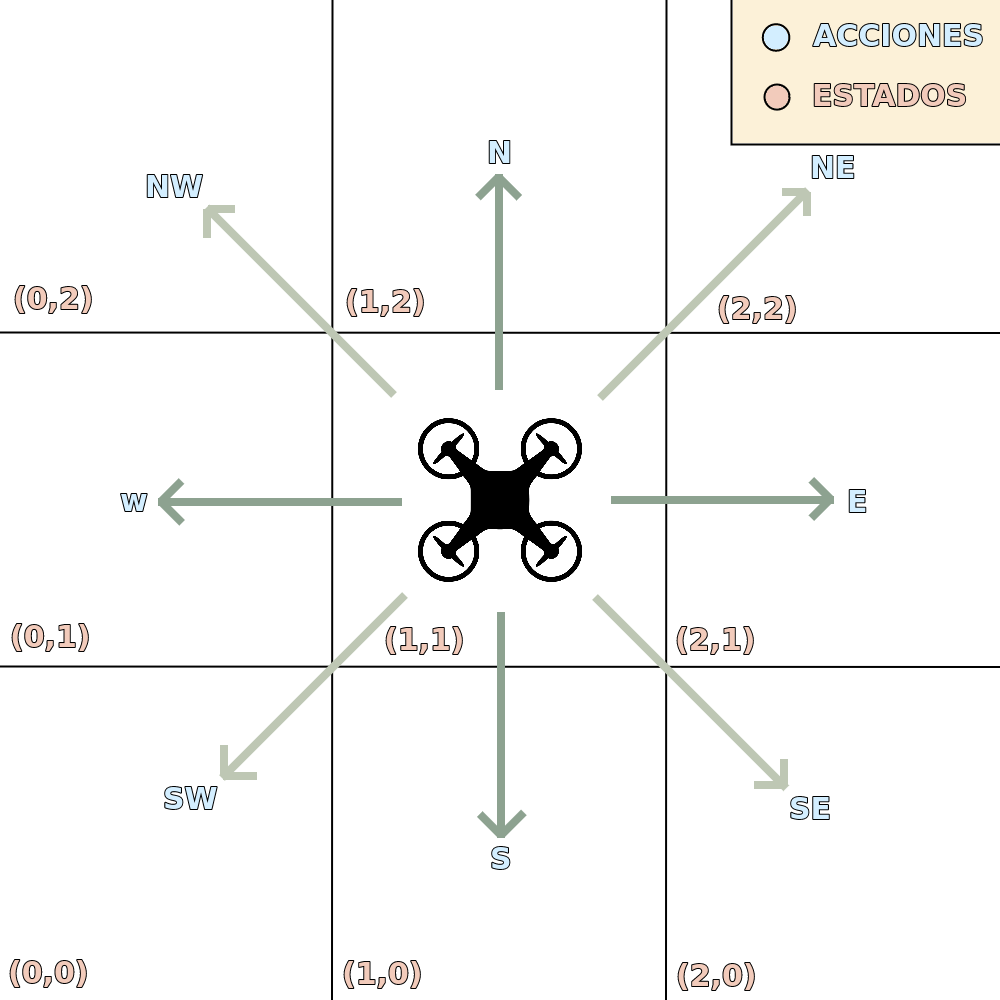
\includegraphics[height=10cm]{imagenes/cap4/6_act_st.png}
    \end{center}
    \caption[Representación de estados y acciones]{Representación de estados y acciones}
    \label{fig:expl_q}
\end{figure}

Como todo algoritmo basado en \ac{RL}, se distinguen dos fases: la fase de entrenamiento, cuyo objetivo es rellenar de forma eficaz la tabla Q, y la fase de inferencia, donde se prueban los resultados obtenidos durante el entrenamiento.\\

\subsubsection{Fase de entrenamiento}
\label{subsubsec:train}

\begin{figure} [t]
    \begin{center}
    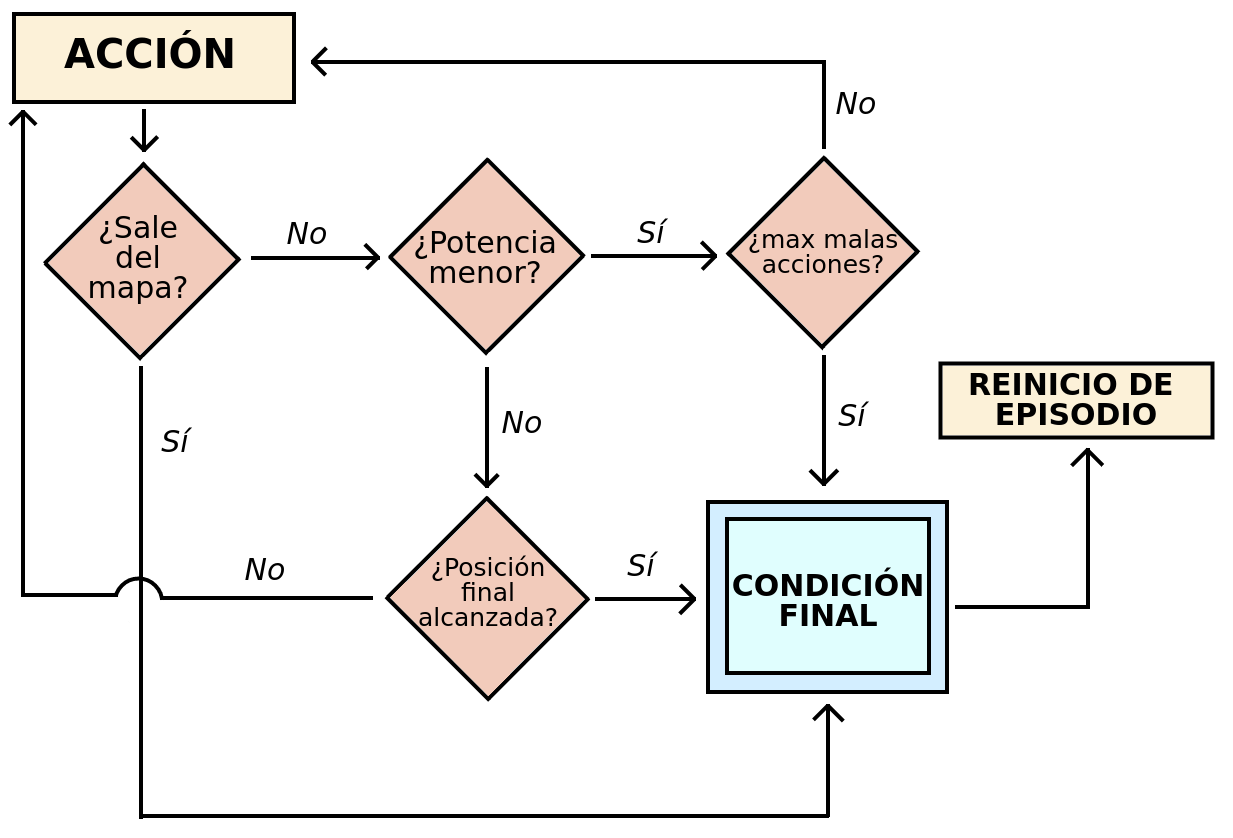
\includegraphics[height=10cm]{imagenes/cap4/11_diagrama_training.png}
    \end{center}
    \caption[Diagrama condición de finalización]{Diagrama condición de finalización}
    \label{fig:training_phase}
\end{figure}

Dentro del entrenamiento, podemos encontrar episodios, que en nuestro caso son las llegadas a la casilla final, o a casillas fuera del mapa definido (adicionalmente se añadió otra condición basada en el número de malas acciones consecutivas, pero de cara a extraer el máximo número de datos posibles para la tabla Q, esta condición no era adecuada, por ello se obvió); y las iteraciones, que se definen literalmente como la realización de una acción. Además, para rellenar el contenido de la tabla, se han definido las pertinentes recompensas y penalizaciones basadas en la diferencia entre la medidas, antes y después de realizar una acción (agregando un pequeño multiplicador a las recompensas negativas), contemplando casos extra, como cuando el dron se sale del mapa, donde se establece una recompensa fija negativa, calculada en proporción al resto de recompensas. Posteriormente, se asignan los valores obtenidos en la tabla Q, haciendo uso de la ecuación~\ref{eq:bellman}, que representa la ecuación de Bellman.
\begin{equation}
    Q(s, a) = (1 - \alpha) \cdot Q(s, a) + \alpha \cdot \left(r + \gamma \cdot \mathrm{max}_{a'} Q(s', a')\right)
    \label{eq:bellman}
\end{equation}
Cabe destacar que, durante el entrenamiento, se especifican una serie de parámetros que han sido ajustados a través de la experimentación, estos son: el número de episodios totales, que repercute directamente en la \emph{fase de exploración} (detallado a continuación); el parámetro $\alpha$, o la tasa de aprendizaje, que afecta a la convergencia de las soluciones durante el aprendizaje; el parámetro $\gamma$, o factor de descuento, que alude a la importancia de las acciones futuras con respecto a las inmediatas; y por último los valores de epsilon ($\epsilon$), que determinan si la acción tomada será aleatoria o extraida de la tabla, esto está directamente asociado a la \emph{fase de exploración}, donde se prioriza la aleatoreidad con el fin de enriquecer con información la tabla Q. En la tabla~\ref{table:params} se muestran los parámetros finales seleccionados durante todos los entrenamientos y experimentos realizados.\\

\begin{table} [t]
    \centering
    \begin{tabular}{ll}
    Número de episodios totales & 10000 \\
    $\alpha$                       & 0'4   \\
    $\gamma$                       & 0'7   \\
    $\epsilon$ (inicial)           & 0'99  \\
    $\epsilon$ (final)             & 0'1   \\
    \end{tabular}
    \caption[Parámetros usados durante todos los entrenamientos]{Parámetros usados durante todos los entrenamientos}
    \label{table:params}
\end{table}

La fase de exploración ocupa un 20\% del número de episodios, de forma lineal, es decir, que cada vez hay más probabilidad de que se tome la acción con mayor peso en la tabla y no de tomar una acción aleatoria (durante el entrenamiento siempre se mantiene cierta posibilidad de tomar una acción arbitraria, para seguir actualizando los datos). Además, para evitar el overfitting (o sobreajuste al entrenamiento, lo que reduciría la adaptabilidad del modelo a escenarios distintos a los del entrenamiento), se han establecido distintos puntos de entrenamiento, para el inicio de los episodios, repartidos de forma uniforme por el mapa, tal y como se mencionará en la sección de métricas.\\

Cabe destacar que, si la acción tomada lleva al dron hacia una condición de final, este finaliza automáticamente el episodio, viajando hacia una nueva posición de entrenamiento y actualizando ciertos parámetros, como es el caso  del parámetro $\epsilon$. La condición de final se aplica siempre tras actualizar los valores intrínsecos en la iteración, tal y como se puede apreciar en la figura~\ref{fig:training_phase}. De forma general, en la actualización de parámetros, se incluye la adición de pesos en la tabla Q según la función de recompensa y un factor aplicado, lo que se traduce en la ecuación~\ref{eq:reward}.
\begin{equation}
    r = (P_f - P_o) \cdot factor
    \label{eq:reward}
\end{equation}
Donde $P_f$ representa el valor leido de la potencia en la nueva posición (tras haber realizado la acción), $P_o$ es el valor de la lectura obtenida antes de realizar la acción, y \emph{factor} equivale a un valor numérico fijo establecido en función de si se le quiere dar más importancia a las recompensas positivas y/o negativas (en nuestro caso es de 1'05 sólo para las recompensas negativas). El orden de magnitud trabajado para esta diferencia se encuentra en torno a las unidades, por ello, se establece el caso de que el dron salga del mapa con una recompensa fija de \emph{``-10''}, que escala al orden de las decenas, lo que nos permite penalizar más dichas decisiones.\\

Una vez realizado el entrenamiento, podemos analizar cómo ha ido a través de la figura~\ref{fig:training_graph}, en este caso, un gráfico triple que nos permite conocer en detalle características del proceso. En concreto, representa tres métricas: el valor de epsilon ($\epsilon$), en el que se distingue la fase de exploración; la recompensa acumulada, que nos permite analizar la convergencia del entrenamiento; y el número de iteraciones, donde se observa que conforme el algoritmo aprende, el número se reduce. Todo ello con respecto a cada episodio. Observamos como en torno al episodio 600 la recompensa acumulada se estabiliza, lo que es una señal de convergencia que indica que el dron alcanza el origen de la señal. Además, conforme se va acabando la fase de exploración, en el episodio 1000, se ve que el número de iteraciones se reduce significativamente, lo que indica menos acciones aleatorias y mayor convergencia hacia una condición de final. En cuanto al tiempo empleado por entrenamiento, usando un portátil ASUS ROG Strix G513QR, con 32 GB de memoria RAM, AMD Ryzen 7 5800h y tarjeta gráfica NVIDIA 3070, tarda aproximadamente 1 hora y 20 minutos, donde 30 minutos son empleados en la fase de exploración.\\

\begin{figure} [t]
    \begin{center}
    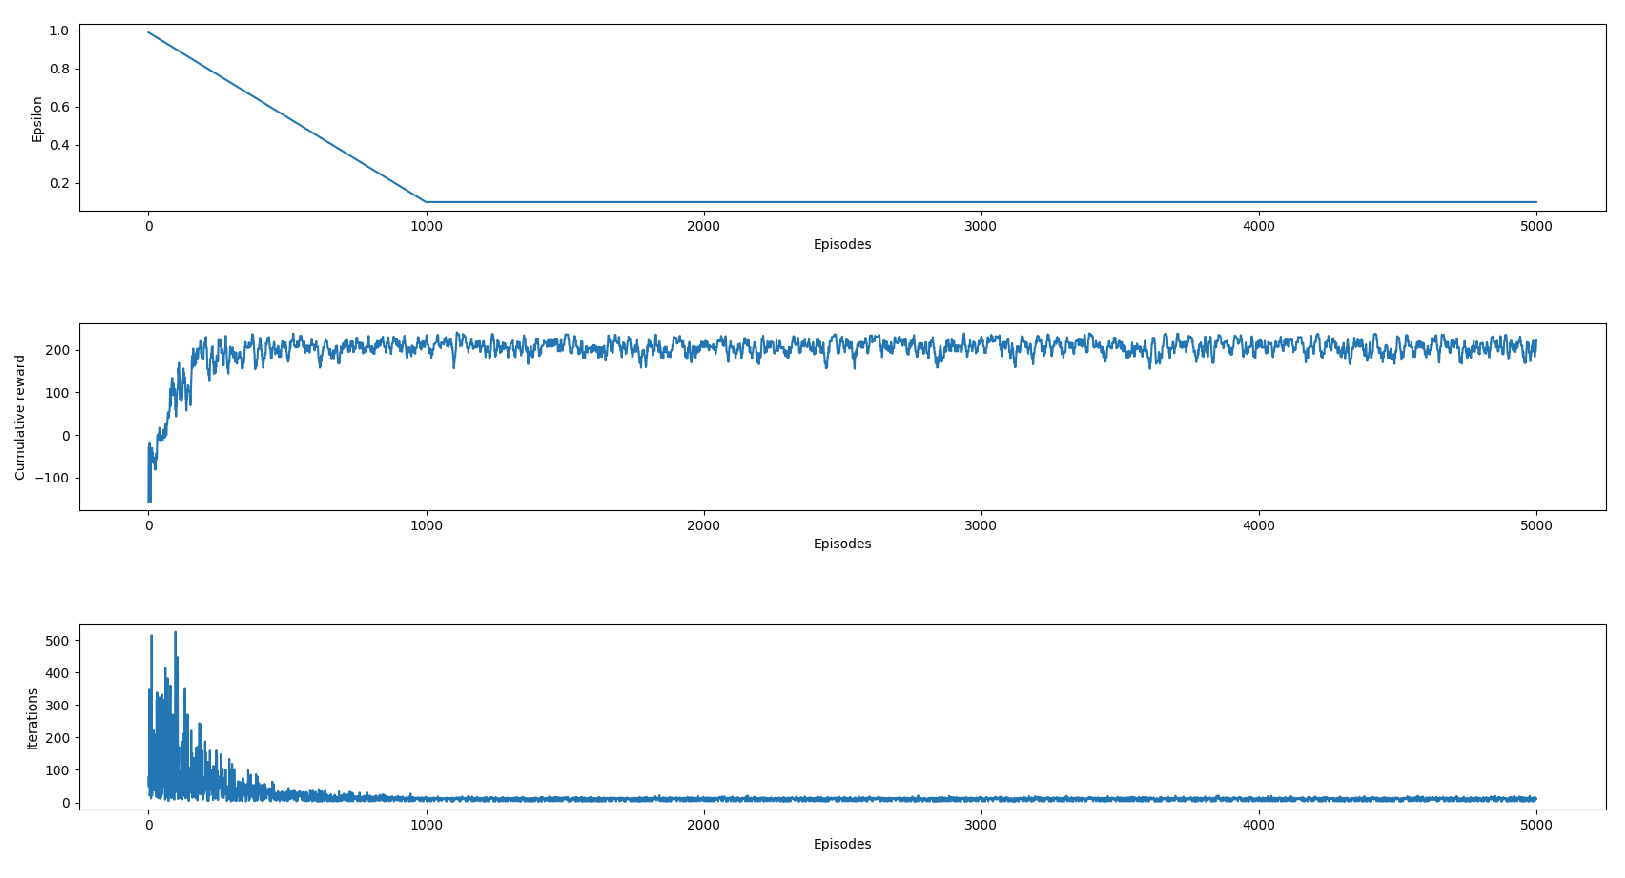
\includegraphics[height=8cm]{imagenes/cap4/14_training_graph.png}
    \end{center}
    \caption[Gráfico de entrenamiento]{Gráfico de entrenamiento}
    \label{fig:training_graph}
\end{figure}

\subsubsection{Fase de inferencia}
\label{subsubsec:test}

Por último, en la \emph{fase de inferencia}, el dron analiza su estado (o sus coordenadas dentro del mapa de calor), y observa la mejor acción disponible dentro de la tabla Q ya rellena. Esto lo realiza hasta que detecta la condición de parada, que se cumple cuando la medida anterior de señal es mayor que la actual y todos los vecinos adyacentes a la mayor de las medidas, poseen señal inferior. Para hacer un correcto análisis, se parte siempre de coordenadas distintas a las que se usaron para entrenar y rellenar la tabla Q.

\subsection{Experimentos y resultados}
\label{subsec:experimentos_sf}

\subsubsection{Experimento 1 - Comparativa de algoritmos para escenarios de distintas dimensiones}
\label{subsubsec:experimentos_1}

Durante todos los experimentos realizados, los parámetros de la señal siempre son los valores por defecto representados en la tabla~\ref{table:compare_graph}, donde sólo varía el tamaño del mapa, que se va modificando según el experimento. Además, cabe destacar que la señal se toma como un punto estático dentro del mapa de calor y con respecto al dron, distinguiendo la posición centrada y la posición cercana a una esquina, que también dependen del experimento. Además, para los todos los entrenamientos realizados, los parámetros usados son los representados en la tabla~\ref{table:params}.\\

\begin{table} [t]
    \centering
    \begin{tabular}{ll}
    Potencia del transmisor & 1 W            \\
    Ganancia del transmisor & 1 W            \\
    Ganancia del receptor   & 1 W            \\
    Frecuencia              & 2'4 GHz (WiFi) \\
    Factor de pérdidas (L)  & 2'4            \\
    Exponente n             & 2              \\
    Resolución              & 1              \\
    \end{tabular}
    \caption[Características de la señal por defecto]{Características de la señal por defecto}
    \label{table:compare_graph}
\end{table}

Primero se ha probado sobre un escenario de tamaño 12x12 metros. Para el transmisor cerca del centro, situada en las coordenadas (5, 5) del \emph{``heatmap''}, extraemos un mapa de puntos donde se muestran las posiciones de entrenamiento o puntos donde el dron despega durante su aprendizaje (representados con una ``X'' roja); inferencia o puntos donde el dron despega para probar lo que ha aprendido (representados por circulos verdes); y del origen del transmisor de la señal (representado por un triángulo azul), así como de los límites del escenario para el mapa de calor (que se distinguen con líneas gruesas). El mapa de puntos obtenido es el representado en la figura~\ref{fig:map_p_center_12}.\\

\begin{figure} [t]
    \begin{center}
    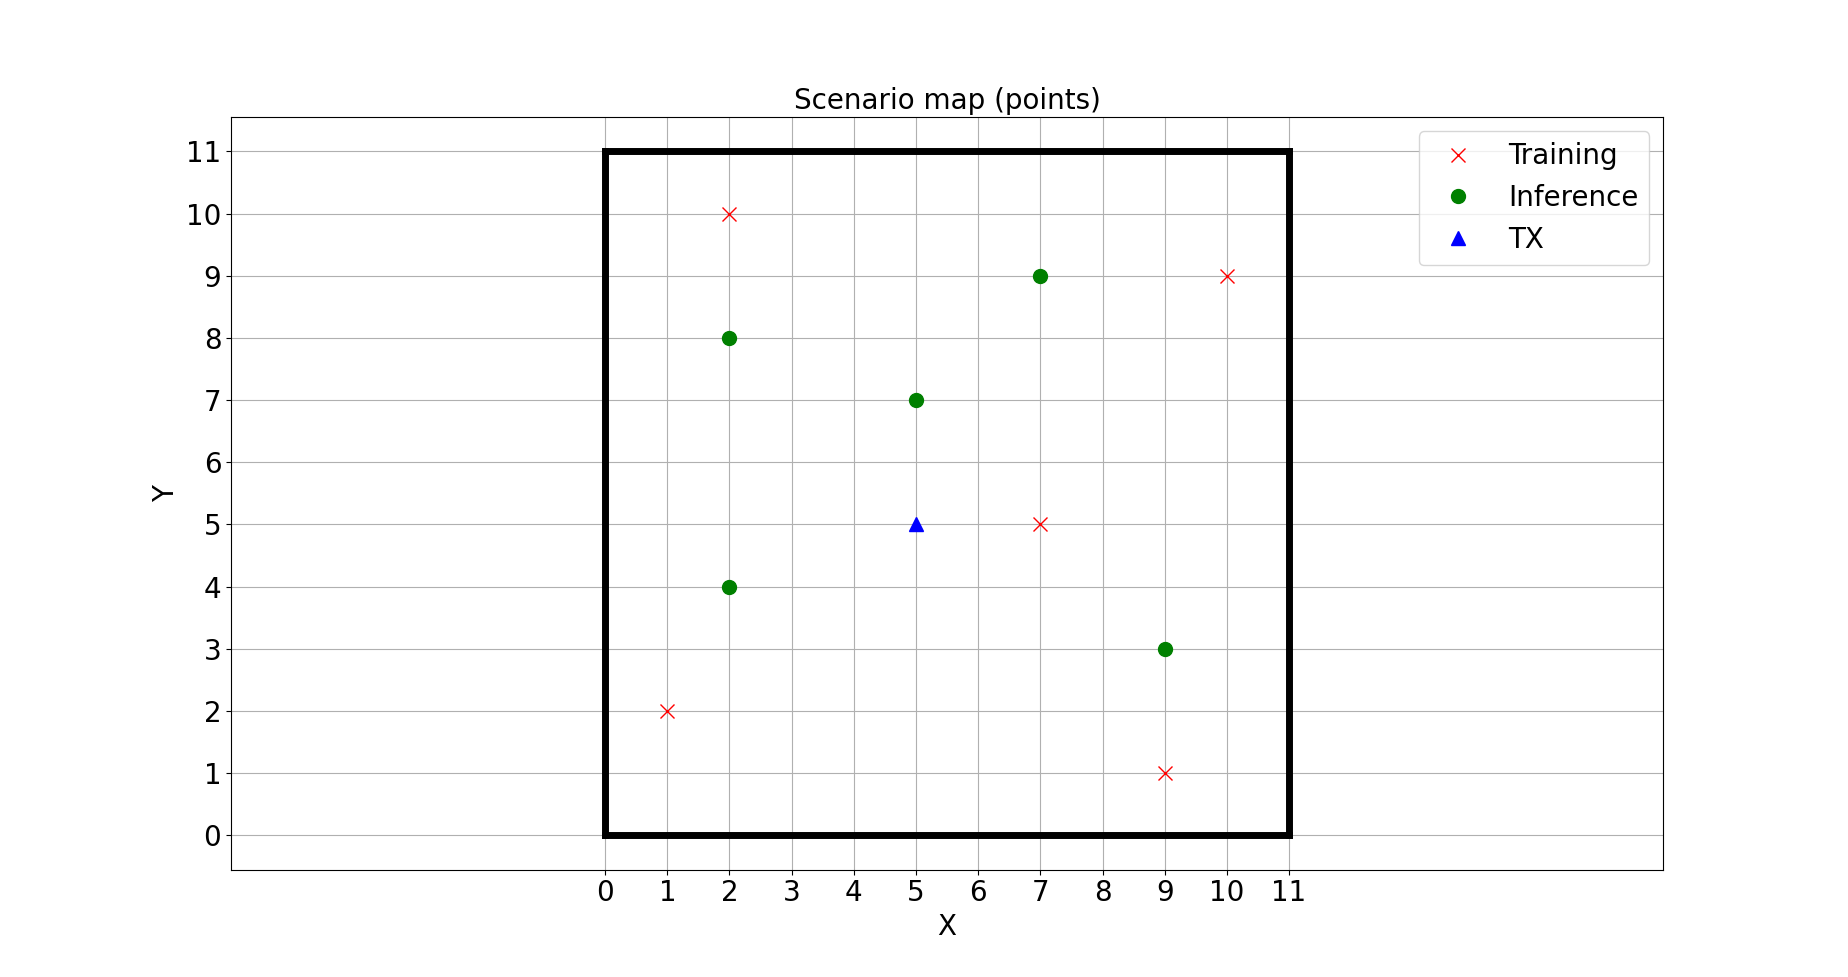
\includegraphics[height=8cm]{imagenes/cap4/17_mapa_p_centro_12.png}
    \end{center}
    \caption[Mapa de puntos (12x12), transmisor centrado]{Mapa de puntos (12x12), transmisor centrado}
    \label{fig:map_p_center_12}
\end{figure}

Los resultados obtenidos, son representados en una serie de gráficas comparativas. En ellas observamos el rendimiento de cada algoritmo, es decir, se analizan tres cosas: el tiempo medio en segundos que tarda el dron desde que despega hasta que vuelve a su posición de despegue; el número medio de iteraciones empleadas para alcanzar el transmisor; y el número medio de movimientos hacía coordenadas donde la potencia de señal es menor y no mayor\footnote[5]{Los datos arrojados han sido guardados en formato \emph{csv}.}.  Para este caso, los resultados obtenidos en la figura~\ref{fig:comp_center_12} arrojan que el algoritmo más eficiente es el de Q-Learning, ya que tarda menos tiempo, realiza menos iteraciones hasta llegar a la meta y tiene un porcentaje inferior de malas acciones. Esto es esperable, debido a que el algoritmo basado en \ac{RL} ha realizado un entrenamiento sobre el que aprende como se propaga la señal, lo que aumenta la exactitud y eficiencia del algoritmo.\\

\begin{figure} [t]
    \begin{center}
    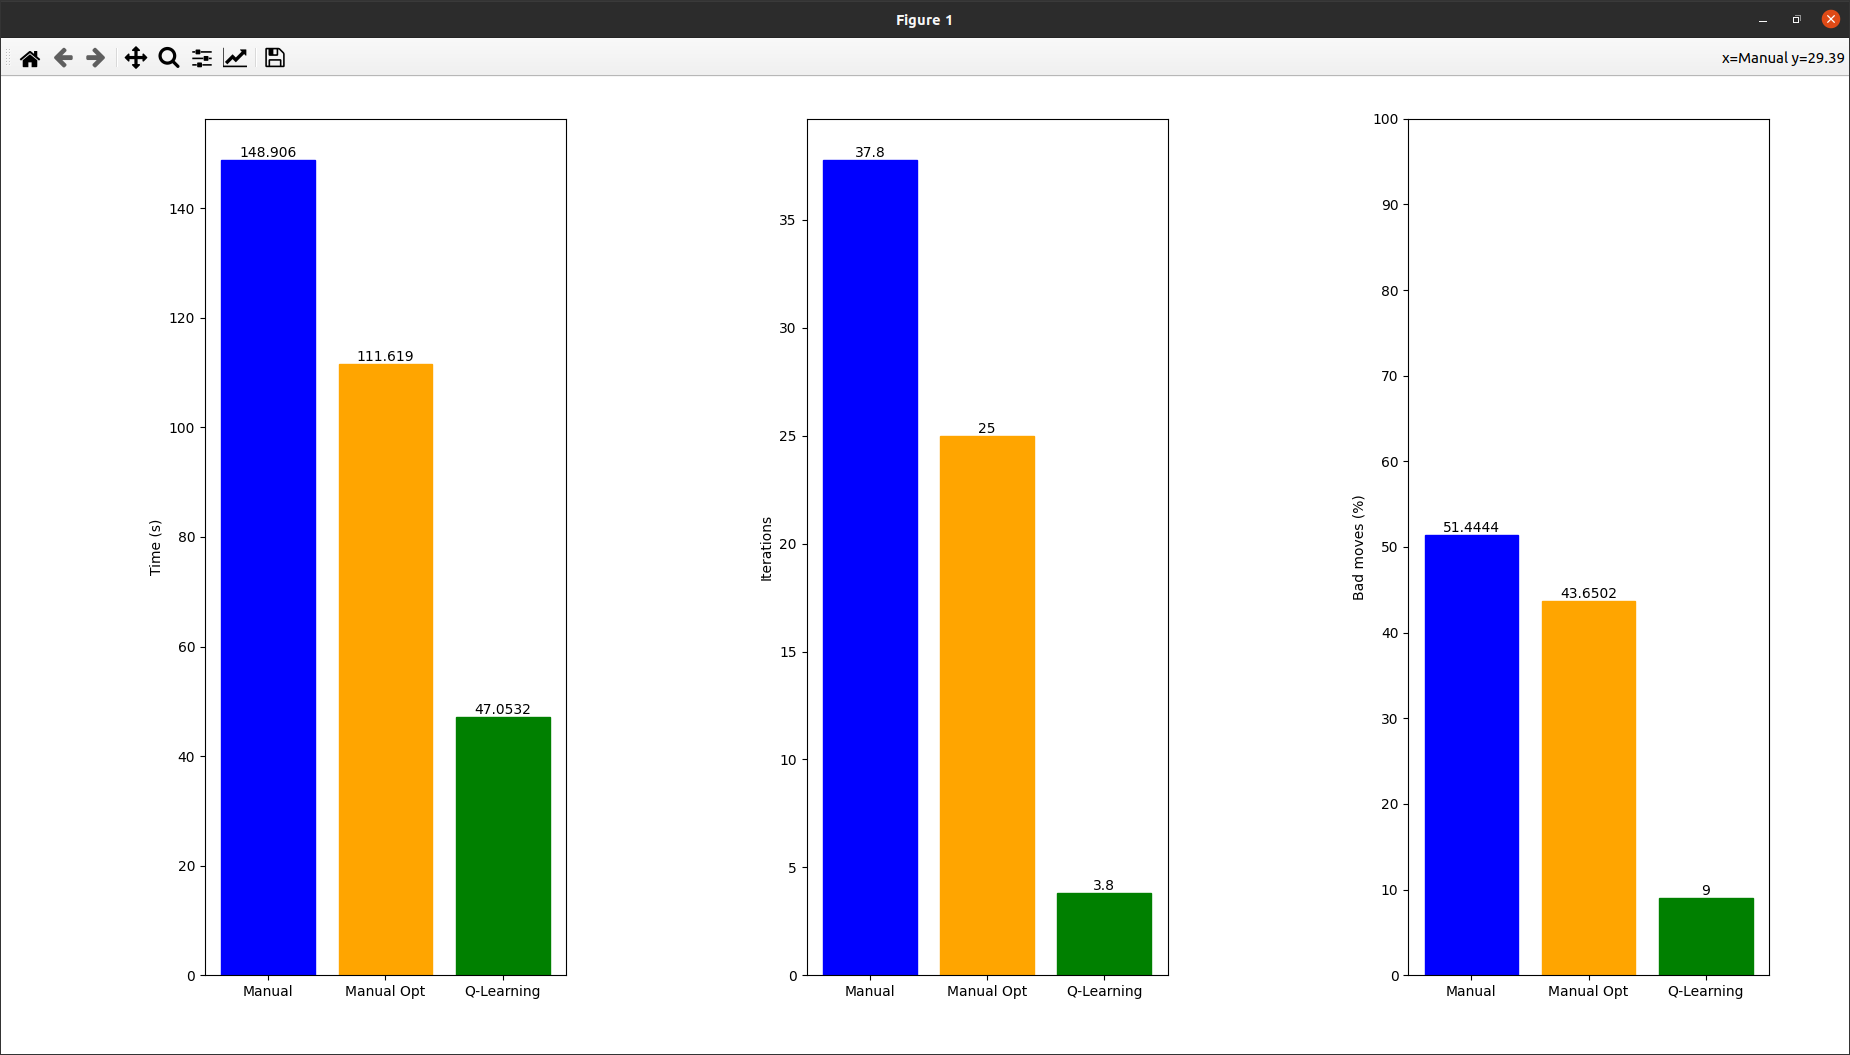
\includegraphics[height=8cm]{imagenes/cap4/18_comp_centro_12.png}
    \end{center}
    \caption[Comparativas (12x12), transmisor centrado]{Comparativas (12x12), transmisor centrado}
    \label{fig:comp_center_12}
\end{figure}

En el caso del transmisor cerca de la esquina, se sitúa en las coordenadas (3, 1) con respecto a las coordenadas del \emph{``heatmap''}, siendo su mapa de puntos el observado en la figura~\ref{fig:map_p_esq_12}.\\

\begin{figure} [t]
    \begin{center}
    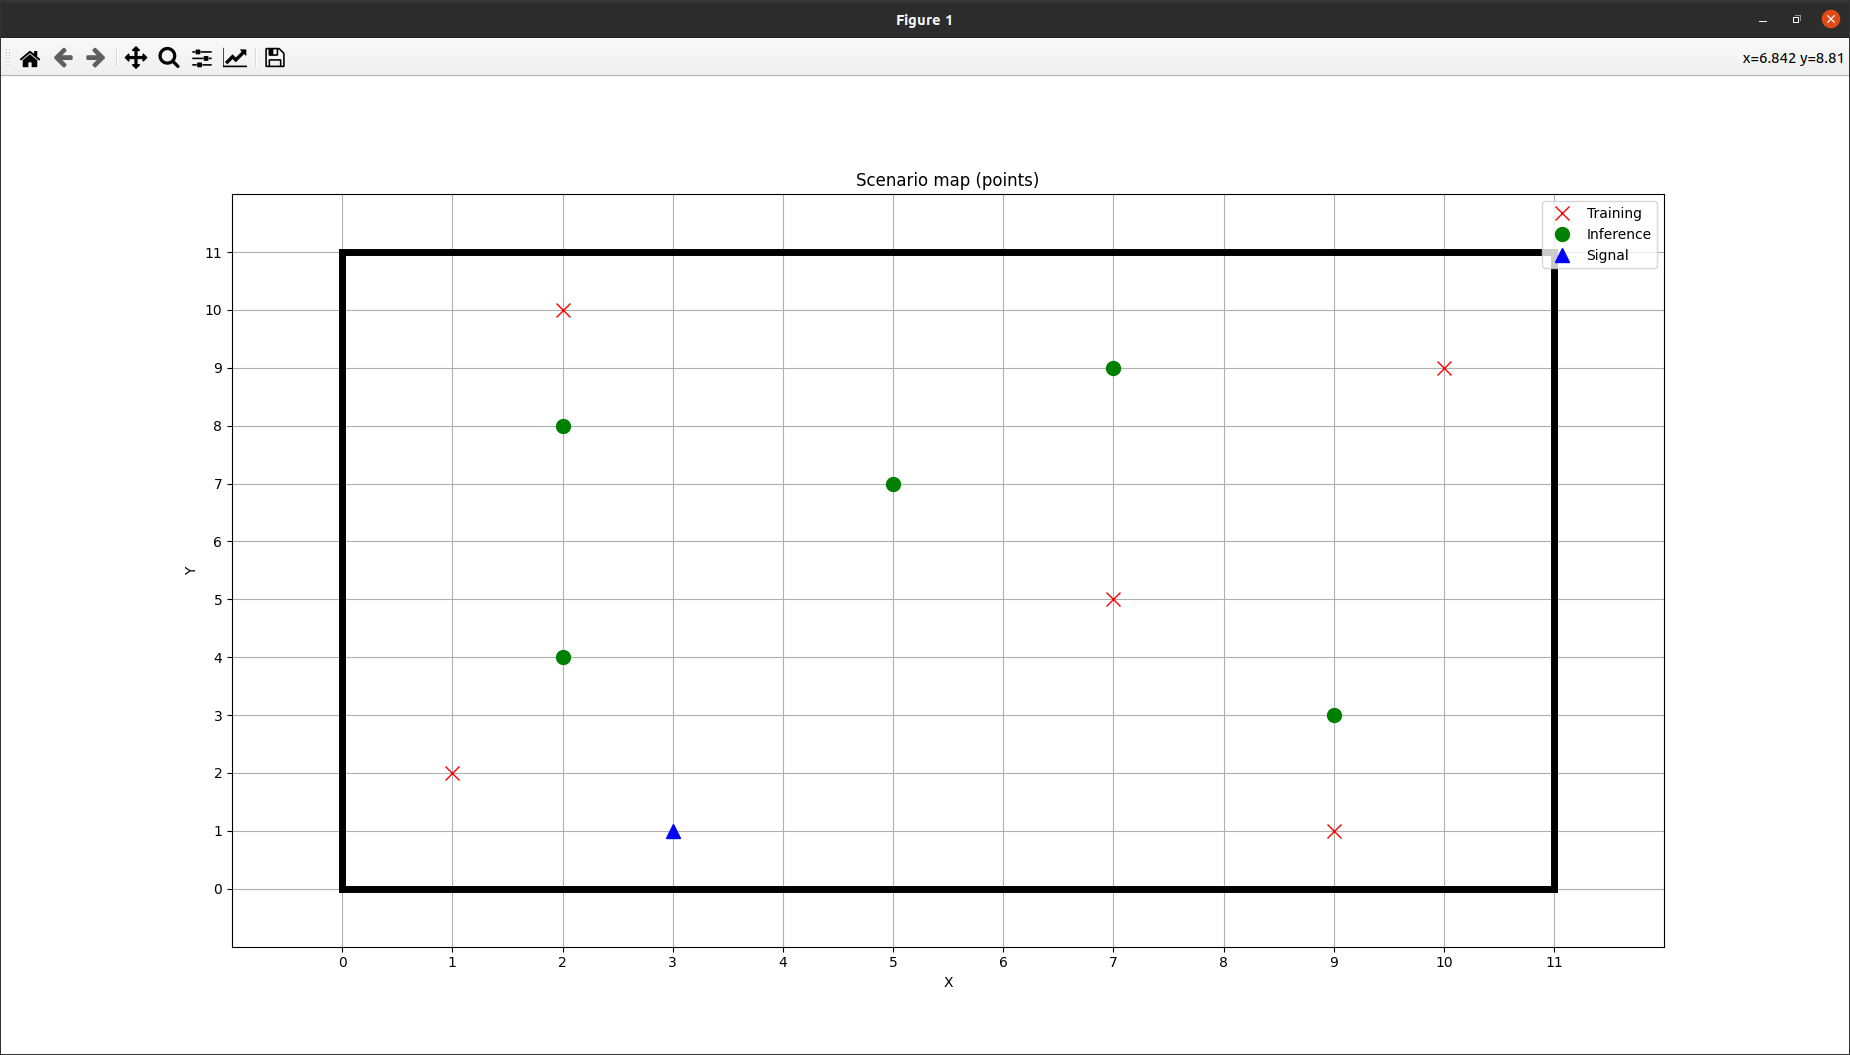
\includegraphics[height=8cm]{imagenes/cap4/19_mapa_p_esq_12.png}
    \end{center}
    \caption[Mapa de puntos (12x12), transmisor en la esquina]{Mapa de puntos (12x12), transmisor en la esquina}
    \label{fig:map_p_esq_12}
\end{figure}

En este caso, se obtiene la misma conclusión que en el escenario anterior, tal y como se aprecia en la figura~\ref{fig:comp_esq_12}.\\

\begin{figure} [t]
    \begin{center}
    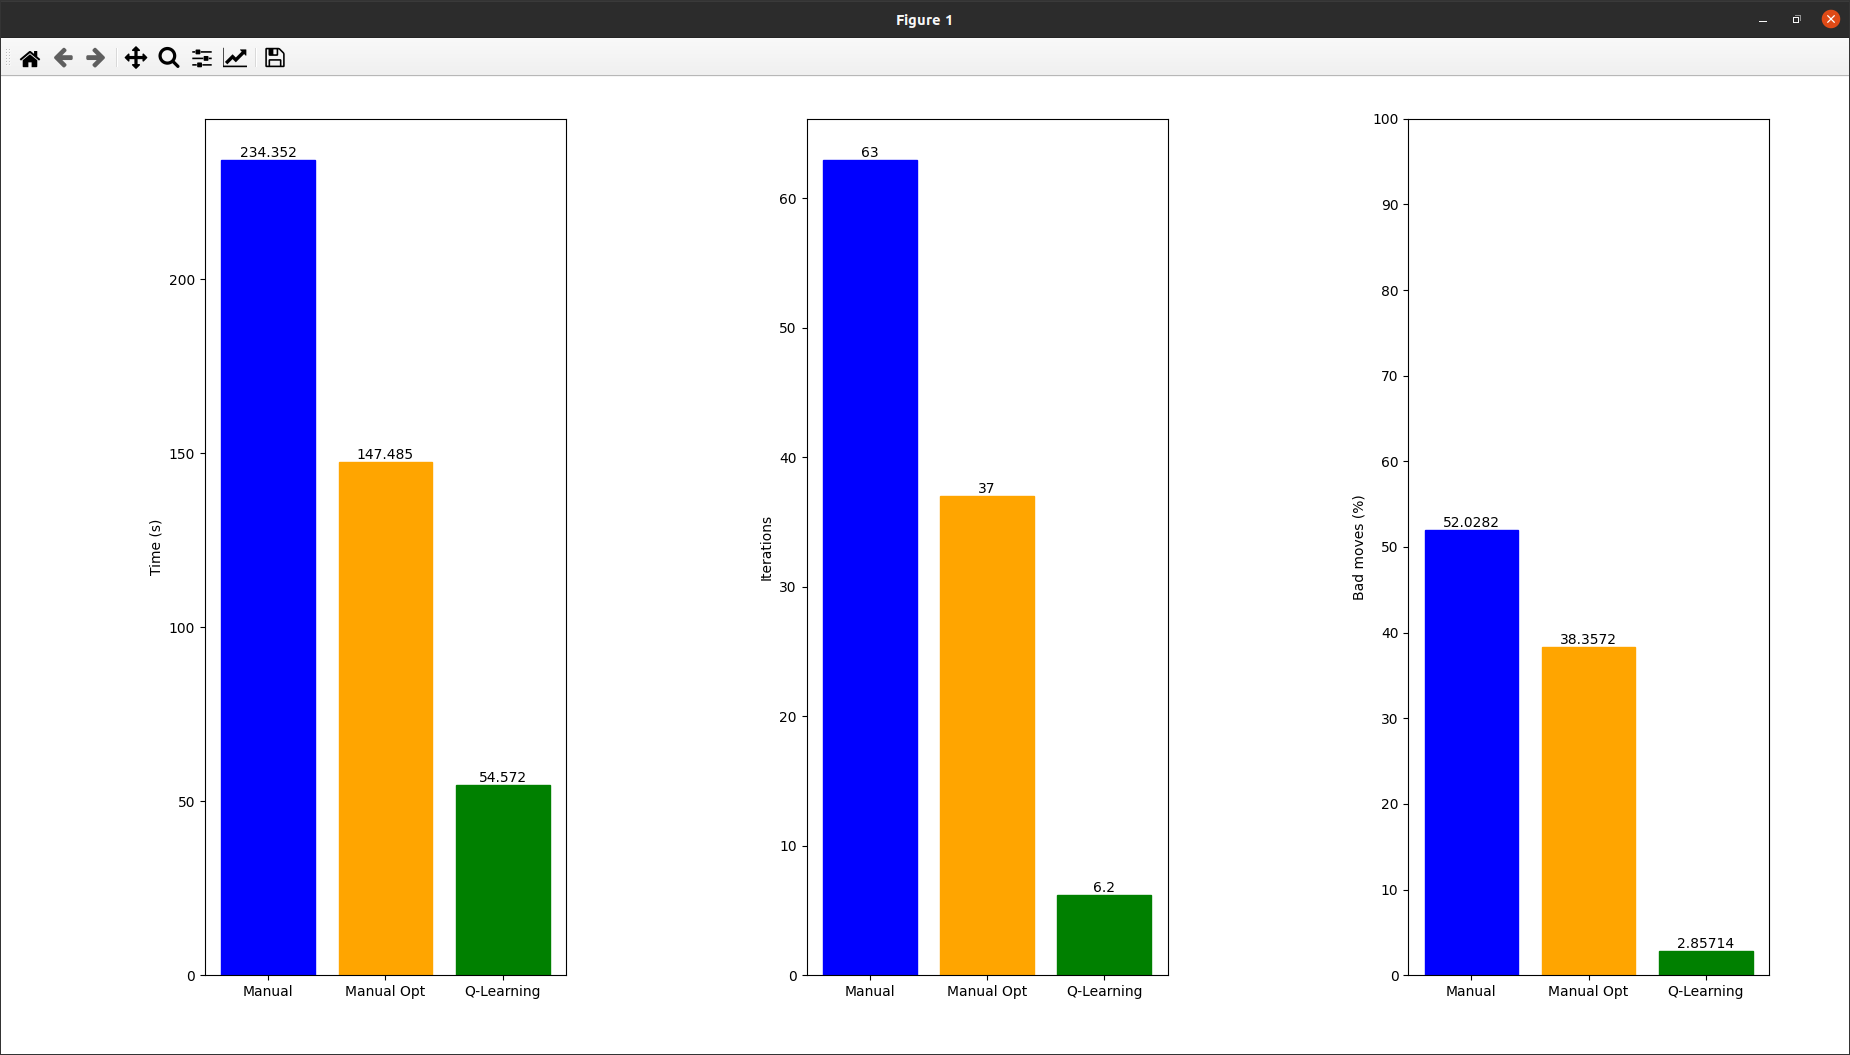
\includegraphics[height=8cm]{imagenes/cap4/20_comp_esq_12.png}
    \end{center}
    \caption[Comparativas (12x12), transmisor en la esquina]{Comparativas (12x12), transmisor en la esquina}
    \label{fig:comp_esq_12}
\end{figure}

Nuevamente, para el escenario de tamaño 30x30, los resultados obtenidos son idénticos, donde, con la salvedad de que el tiempo empleado es mayor y el número de iteraciones también, se concluye que el algoritmo de \ac{RL} es el mejor en todos los casos.\\

\subsubsection{Experimento 2 - Desempeño del algoritmo Q-Learning para dos señales distintas}
\label{subsubsec:experimentos_1}

En este caso, se ha realizado un experimento en el cual se entrena al modelo de Q-Learning con los parámetros especificados en la tabla~\ref{table:params}, donde el transmisor emite con las características de señal mencionadas en la tabla~\ref{table:compare_graph} (en gráficas comparativas hace referencia a \emph{``Q-Learning''}). A continuación se realiza inferencia, y posteriormente se modifican las características de la señal, aumentando la potencia del transmisor al doble (2 W) y cambiando la frecuencia (de 2'4 GHz a 5 GHz), de modo que en las gráficas comparativas se nombra como \emph{``Q-Learning 2''}. Nuevamente se realiza inferencia y se extraen resultados. Las coordenadas en las que se sitúa el transmisor están en (5, 3) y no son modificadas en ningún momento. Además, los puntos de entrenamiento seleccionados se pueden ver en el mapa de puntos de la figura~\ref{fig:map_p_diff_30}.\\

\begin{figure} [t]
    \begin{center}
    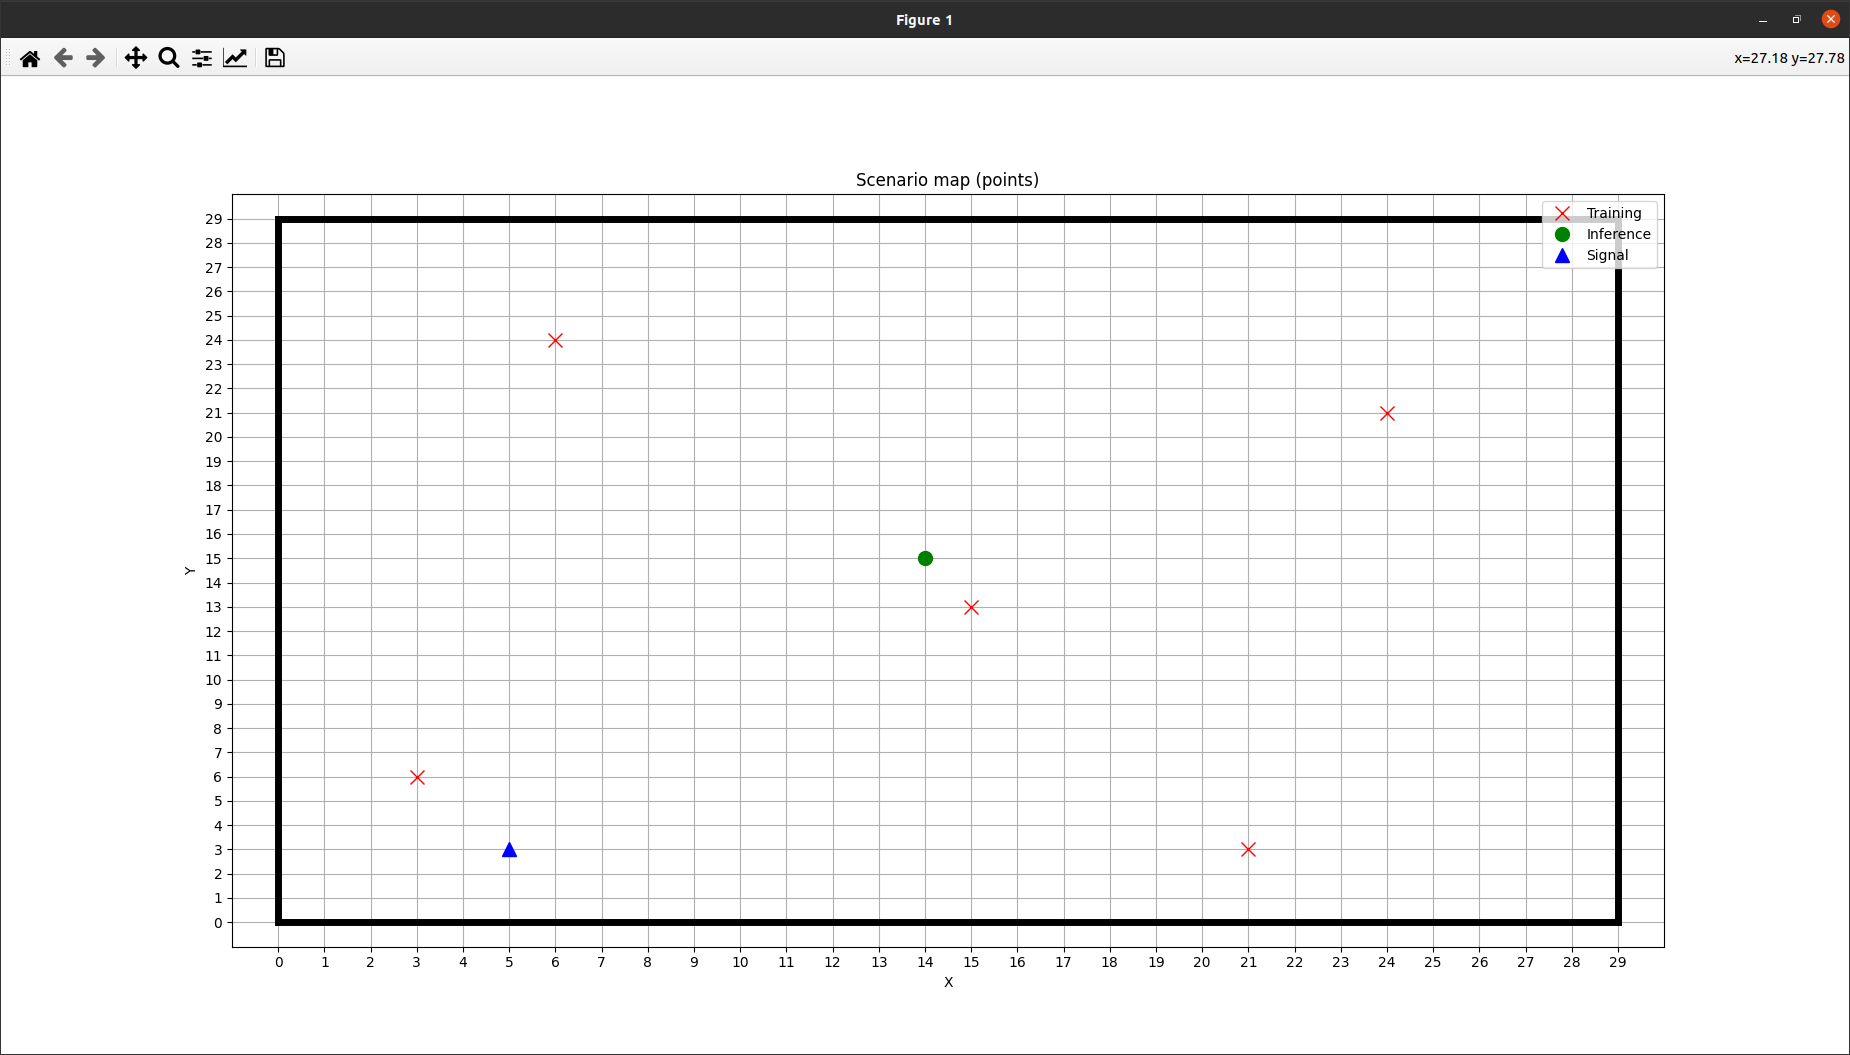
\includegraphics[height=8cm]{imagenes/cap4/25_mapa_p_diff.png}
    \end{center}
    \caption[Mapa de puntos del escenario planteado (30x30)]{Mapa de puntos del escenario planteado (30x30)}
    \label{fig:map_p_diff_30}
\end{figure}

Para este caso, el problema se resuelve de igual forma para ambos casos, con una cierta variación irrelevante en la métrica temporal, derivada probablemente de la propia simulación, lo que se puede concluir como que el modelo aprende como se propaga la señal, independientemente de las características de la misma. Como se puede observar en la figura~\ref{fig:comp_diff_30}, se muestran las gráficas comparativas y un gráfico de trayectorias (figura~\ref{fig:12_traj}), que representa el camino seguido por el dron al aplicar la inferencia en ambos casos.\\

\begin{figure} [t]
    \begin{center}
    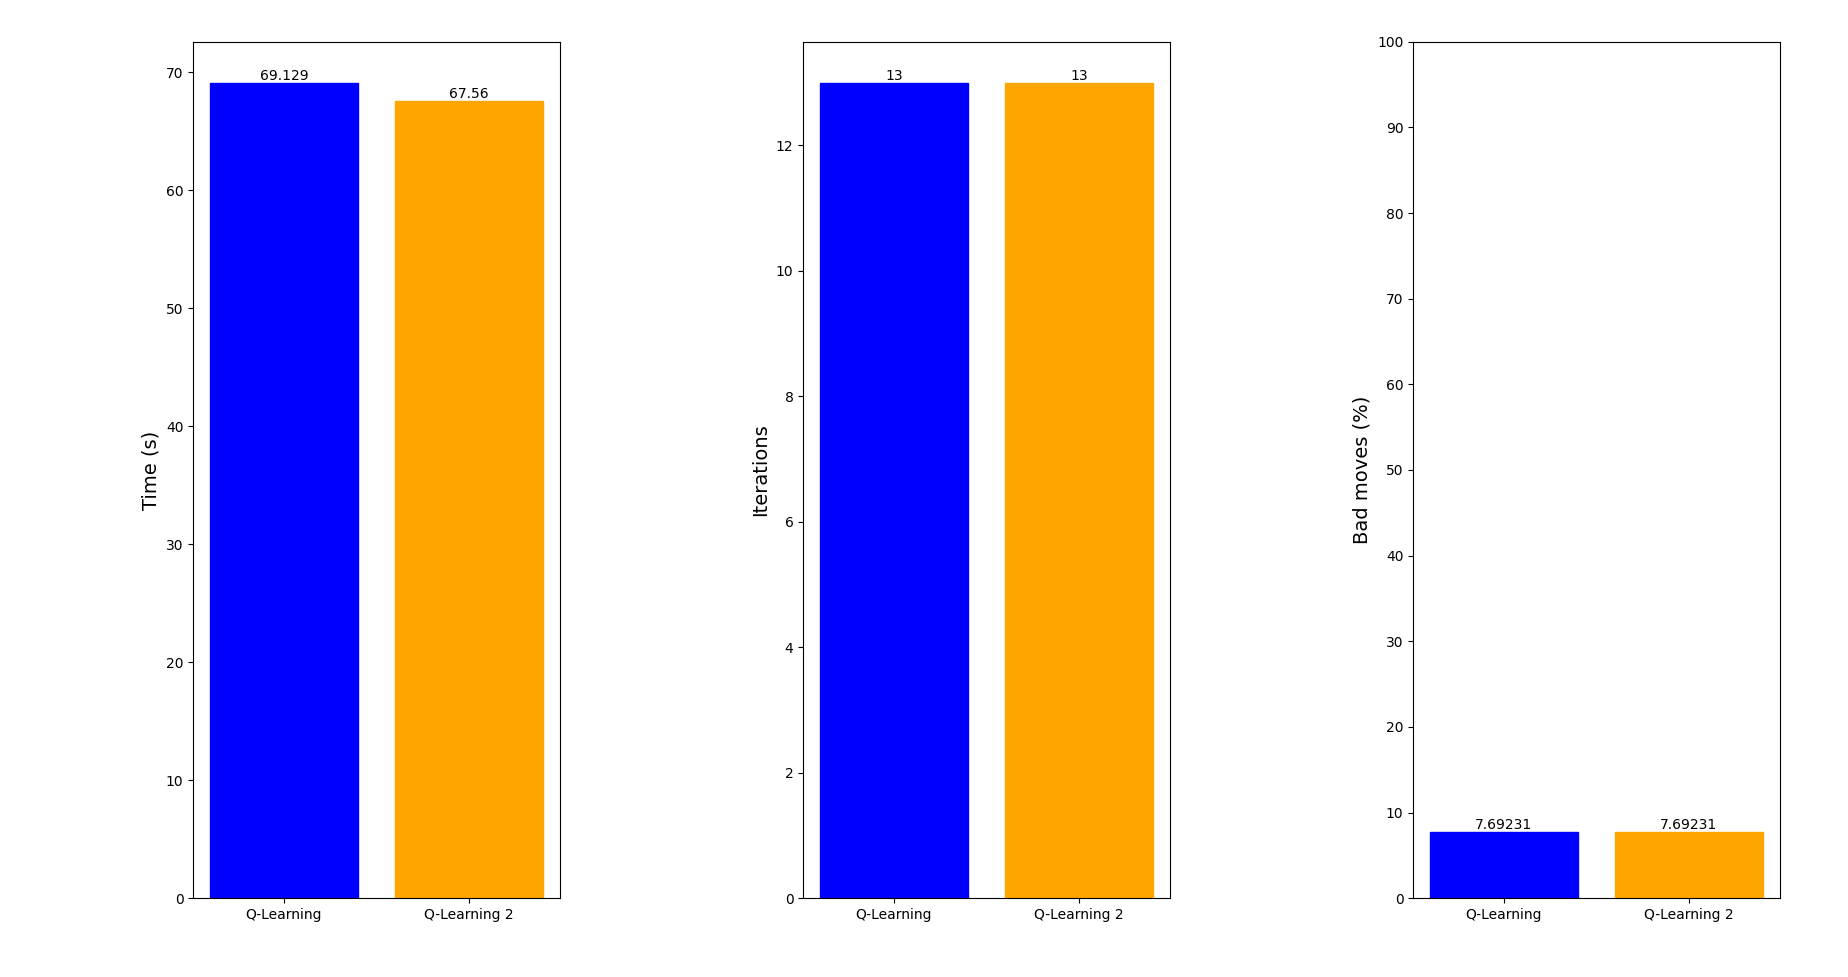
\includegraphics[height=7.5cm]{imagenes/cap4/26_comp_diff.png}
    \end{center}
    \caption[Comparativas (30x30), escenario planteado]{Comparativas (30x30), escenario planteado}
    \label{fig:comp_diff_30}
\end{figure}

\begin{figure} [t]
    \begin{center}
    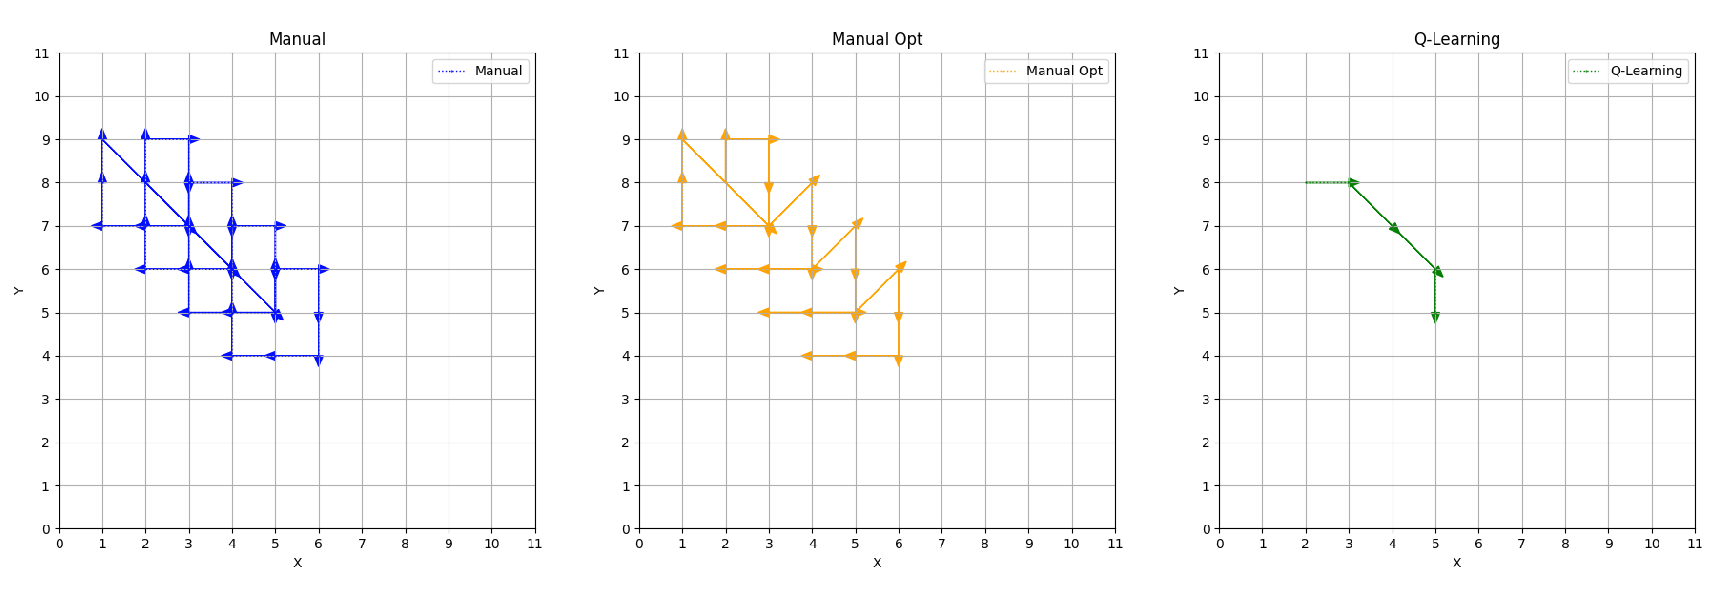
\includegraphics[height=8cm]{imagenes/cap4/13_trayectorias_12.png}
    \end{center}
    \caption[Trayectorias seguidas durante la inferencia]{Trayectorias seguidas durante la inferencia}
    \label{fig:12_traj}
\end{figure}

\section{Comportamiento sigue señal basado en \ac{RF} en un entorno dinámico}
\label{sec:signal_follow_obs}

\subsection{Introducción al problema}
\label{subsec:intro_sfo}

El escenario planteado anteriormente, es una aproximación poco realista, es decir, en un entorno real se esperan perturbaciones y obstáculos. Por ello, se ha implementado un escenario con muros que distorsionan la señal.\\

Inicialmente, se ha establecido el mapa a mano, es decir, se han sobreescrito los valores degradados de la señal sobre el mapa original para simular un mapa con obstáculos.\\

\subsection{Algoritmos}
\label{subsec:algoritmo_sfo}

En cuanto a los algoritmos empleados, se parte de la idea de realizar un entrenamiento normal sin obstáculos, y ajustar el comportamiento a las situaciones emergentes.\\

Por ello se distinguen dos casos:

\begin{enumerate}
    \item \emph{El dron vuela por encima de la altura del obstáculo}: es decir, el dron navega por una zona con interferencias pero a una altura donde no exista colisión.
    \item \emph{El dron vuela a la misma altura que el obstáculo}: donde según que camino se escoja puede existir colisión.
\end{enumerate}

\subsection{Experimentos y resultados}
\label{subsec:experimentos_sfo}

Por ello, se observa que para el primer caso donde el dron sobrevuela cualquier muro, no existe inconveniente, puesto que el dron toma el camino que tomaría si no hubiera obstáculos. Esto es debido a que en inferencia, tan solo se tiene en cuenta su posición con respecto al mapa de calor, y por tanto no identifica si hay o no obstáculos. Sin embargo, sí es relevante a la hora de abordar la condición de finalización, ya que al modificar el mapa de señal, se pueden dar falsos positivos y generar mínimos locales. Por ello, se ha empleado una técnica que analiza, por pares, las coordenadas visitadas, de modo que se tiene la coordenada actual y la nueva, y por iteración se compara con la siguiente actual y la siguiente nueva, y si coinciden, se cumple la condición pasando al análisis de los vecinos cercanos, como en todos los casos anteriores. Por último cabe destacar que esta condición funciona para desplazamientos de 1 m, o dicho de otro modo, de celdilla en celdilla.\\

En el otro escenario, donde el dron vuela a la altura de los obstáculos, se debe implementar un método de detección de obstáculos. En general, se puede generar un caso realista usando un láser LiDAR o una cámara 3D, pero para simplificar el problema, se ha empleado la información del mapa realizando una simulación del comportamiento que tendría un sensor genérico de este tipo. Por ello, primero se prueba excluyendo las acciones que desemboquen en colisión, donde se presupone que el entrenamiento evitará acciones que alejen al dron de la señal, tal y cómo se observa en la figura~\ref{fig:pseudosensor}.\\

\begin{figure} [t]
    \begin{center}
    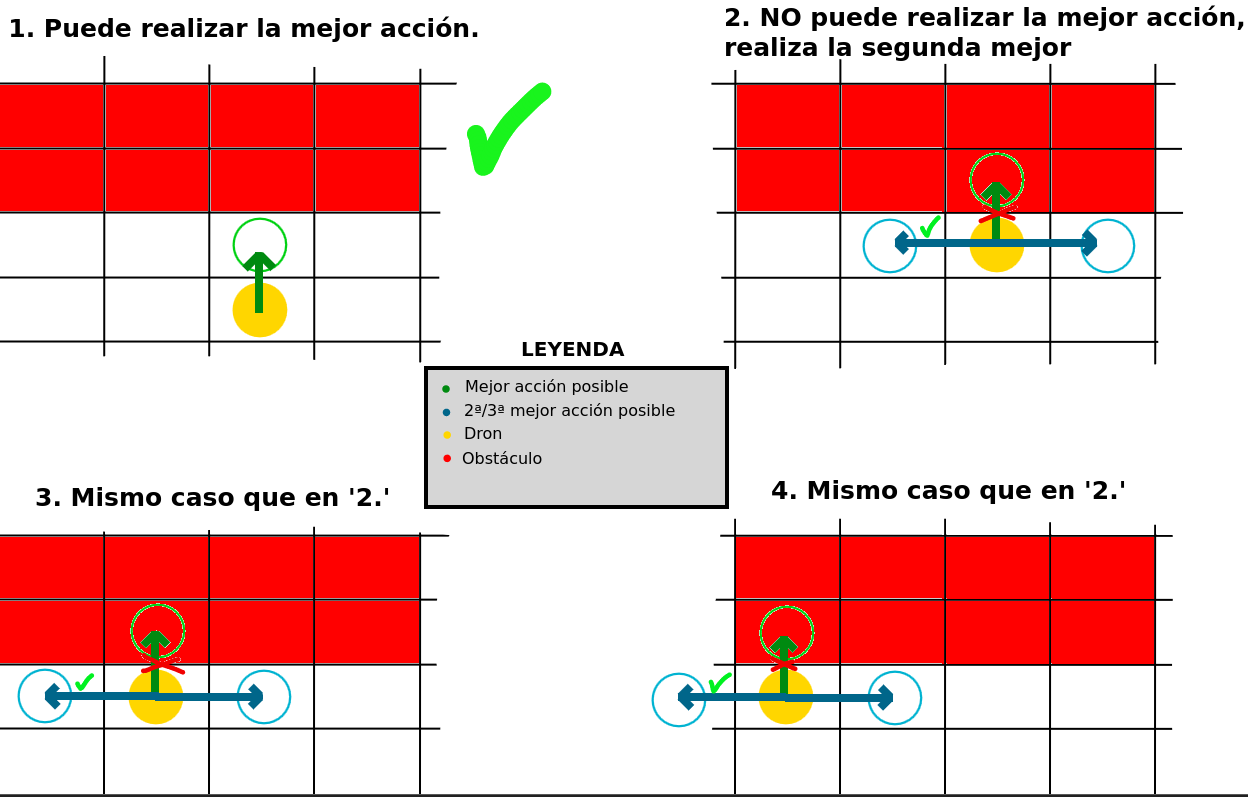
\includegraphics[height=9cm]{imagenes/cap4/28_pseudosensor.png}
    \end{center}
    \caption[Simulación de sensor para obstáculo]{Simulación de sensor para obstáculo}
    \label{fig:pseudosensor}
\end{figure}

Sin embargo, los resultados no son concluyentes, de modo que en ocasiones sortea el obstáculo, pero en otras simplemente retrocede o alcanza un mínimo local. De este modo, y volviendo a la conclusión extraida del primer escenario, se ve la necesidad de aplicar un comportamiento híbrido, de modo que se navegue hacia la señal, hasta topar con un obstáculo lo suficientemente cercano, como para que cambie el modo de actuación para evitarlo. Una vez sorteado, se vuelve modo de navegación normal, hasta llegar a la señal o a otro obstáculo.\\

Por ello, se opta por emplear un algoritmo basado en \ac{VFF}, que consiste en generar un comportamiento basado en vectores de fuerzas virtuales, de modo que se alcanzen subobjetivos cercanos, evitando colisiones con obstáculos. Para nuestro caso concreto, se ha decidido adaptar de modo que: los obstáculos son dispuestos en el mapa por celdillas ocupadas, de modo que cada celdilla genera un vector inversamente proporcional a la distancia, desde la celdilla a la posición del dron, generando un vector de repulsión; los subobjetivos que generarían el vector de fuerza atractiva, son sustituidos por un vector basado en la tendencia seguida por el dron, durante la navegación basada en Q-Learning, es decir, se obtiene un vector unitario resultante de todas las posiciones visitadas por el dron, previamente. Todo esto, se ajusta siguiendo la ecuación~\ref{eq:vff}, que traducido a comandos para el dron son velocidades en x, y, ya que es lo que mejor se ajusta al comportamiento reactivo buscado.
\begin{equation}
    F_{res} = \alpha \cdot F_{atr} + \beta \cdot F_{rep}
    \label{eq:vff}
\end{equation}
Donde tras el ajuste por experimentación, $\alpha$ (que determina la importancia que tendrá la fuerza atractiva en la ejecución) toma el valor de 2'5, y $\beta$ (que por contra determina la importancia de la fuerza repulsiva) toma el valor de 0'05. Adicionalmente, es necesario comentar un problema derivado del diseño a la hora de simular el escenario. A causa de que el transmisor se sitúa esquinado y el obstáculo también, y dado que el dron solo actuaba sobre el muro, si el algoritmo \ac{VFF} desplazaba al dron fuera de las coordenadas del mapa de calor, se generaban comportamientos impredecibles (lo cual en la realidad no sucedería, ya que la señal se propagaría en todas direcciones). Para solucionarlo, se agregaron muros virtuales que actúan como obstáculos, con el fin de delimitar estas áreas fuera del mapa de calor. El resultado final es satisfactorio, ya que se consigue navegar hacia la señal, evitando obstáculos. En la figura~\ref{fig:hybrid}, se puede ver una representación gráfica del escenario y su funcionamiento, donde se dispone un muro, el transmisor y el algoritmo funcionando en ambos modos.

\begin{figure} [t]
	\centering
	\subfigure[Q-Learning]{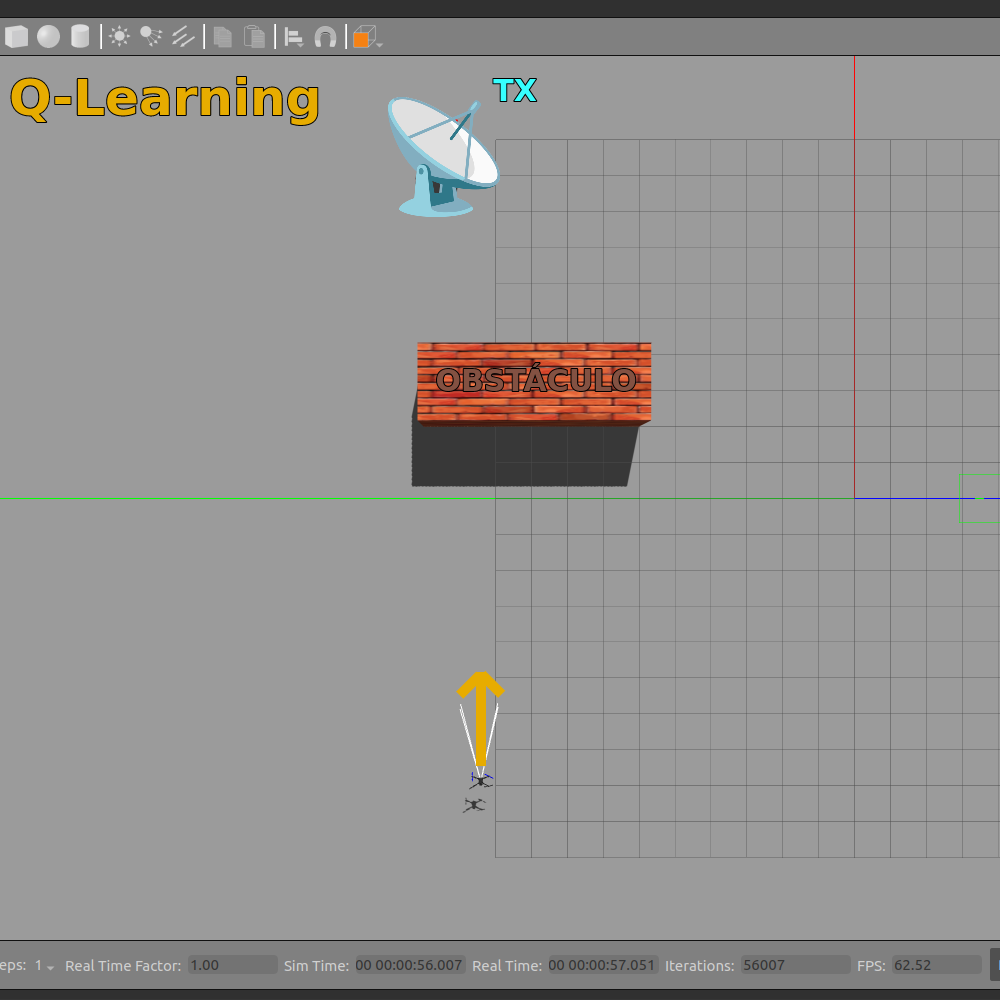
\includegraphics[height=10cm]{imagenes/cap4/0_ql.png}}
	\quad
	\subfigure[VFF]{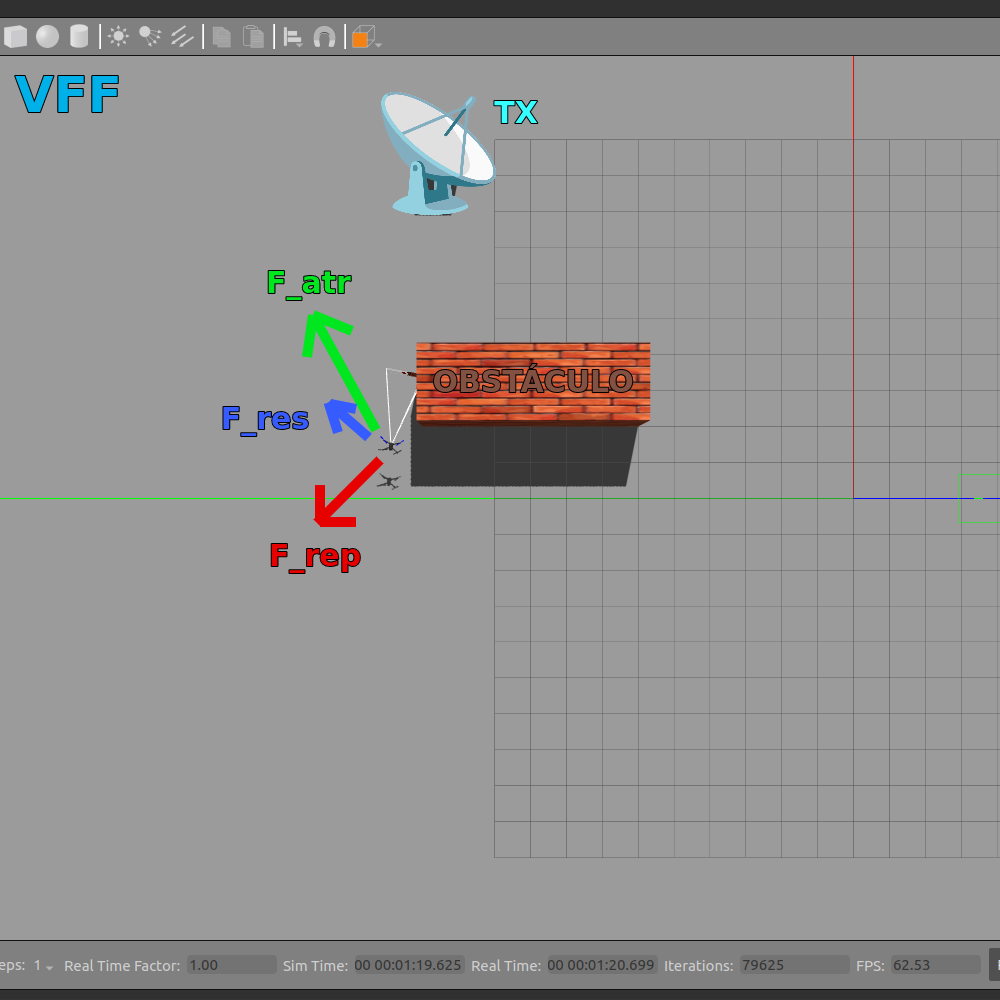
\includegraphics[height=10cm]{imagenes/cap4/0_vff.png}}
	\caption{Enfoque híbrido}
	\label{fig:hybrid}
\end{figure}
